%%%%%%%%%%%%%%%%%%%%%%%%%%%%%%%%%%%%%%%%%
% Masters/Doctoral Thesis
%
% %%%%% IMPORTANT %%%%%
% 1) Edit Front/vars.tex
% 2) Compile Front/main.tex
% 3) Edit vars.tex
% 4) Edit precontent.tex
%
% BEFORE ANYTHING ELSE
% You can also set some interesting stuff in the preamble.tex file
% If you know what you're doing.
%%%%%%%%%%%%%%%%%%%%%%%%%%%%%%%%%%%%%%%%%

% The default font size and two-sided printing
% For a one-sided printing change the flag "twoside" to "oneside"
\documentclass[11pt, oneside, table,xcdraw]{Thesis}


%-------------------------------------------------------------------------
%   PREAMBLE AND SETTINGS
%-------------------------------------------------------------------------
% Add the preamble. You can change various settings in here
%-------------------------------------------------------------------------
%	PACKAGES AND OTHER DOCUMENT CONFIGURATIONS
%-------------------------------------------------------------------------

\usepackage{rotating}
\usepackage{pdflscape}
\usepackage{adjustbox}

% Include pdf pages in the document
% Necessary to include the front pages (cover and etc.)
\usepackage{pdfpages}

% For the cover page
\usepackage{tikz}

% Fix top page geometry on long titles
\setlength{\headheight}{14pt}  %Try fix error

% Language hyphenation and typographical rules
\usepackage[portuguese,english]{babel}
%Custom hyphenization
\hyphenation{Py-thon}
\hyphenation{Ju-py-ter}
\hyphenation{Ma-the-ma-ti-ca}

% Inline quotes
% added for \begin{displayquote}
\usepackage[autostyle]{csquotes}

% Bibliography setup
% Use the natbib reference package - read up on this to edit the reference
% style; if you want text (e.g. Smith et al., 2012) for the in-text references
% (instead of numbers), remove 'numbers'
\usepackage[square, numbers, comma, sort&compress]{natbib}
\bibliographystyle{IEEEtranN}  % I actually quite like this one
% \bibliographystyle{apsrev4-1-etal} % With emphasized titles. ORIGINAL
% Prevent that the first citation is in the ToC
\usepackage{notoccite}
\setlocalecaption{english}{bib}{References}


% Interesting float placements (like 'H') and custom float types
\usepackage{float}
% Text wrapped around pictures
% https://pt.sharelatex.com/learn/Wrapping_text_around_figures
\usepackage{wrapfig}
% Force float barriers, use as \FloatBarrier
\usepackage[section]{placeins}
% Place floats *above* footnotes
\usepackage[bottom, perpage, symbol]{footmisc}
% Set default float placement
\makeatletter
\renewcommand{\fps@figure}{tbph}
\renewcommand{\fps@table}{tbph}
\makeatother

% Pretty colours
\usepackage{xcolor}
% \usepackage{color} % Deprecated by xcolor

% SVGs with Inkscape and PDF+LaTeX
% https://tex.stackexchange.com/questions/473994/svg-and-inkscape
\usepackage[inkscapearea=page]{svg}
% Specifies the directory where vector are stored
\svgpath{{Svgs/}}

% Graphics stuff
\usepackage{graphicx}  % invoked by svg
% Specifies the directory where pictures are stored
\graphicspath{{Figures/}}

% For sub-figures and stuff
\usepackage{caption}
\usepackage{subcaption}

% Math stuff
\usepackage{amsmath} % Interesting environments
\usepackage{amssymb} % Interesting symbols
\usepackage{commath} % Interesting macros
\usepackage{braket} % Dirac bra-ket and set notations
\usepackage{mathpazo} % Math font (palatino for Computer Modern on math)
\usepackage{mathtools} % Mathematical tools to use with amsmath
\setstretch{1.5}
% Math alphabet
\DeclareMathAlphabet{\pazocal}{OMS}{zplm}{m}{n}
\newcommand{\Sa}{\pazocal{S}}
\newcommand{\Ua}{\pazocal{U}}
\newcommand{\Ha}{\pazocal{H}}
\newcommand{\Fa}{\pazocal{F}}
\newcommand{\Ia}{\pazocal{I}}
\newcommand{\Ea}{\pazocal{E}}
\newcommand{\ja}{\pazocal{J}}
%Custom math operators
\DeclareMathOperator*{\meshgrid}{meshgrid}
% Floor and ceiling of numbers
\DeclarePairedDelimiter\ceil{\lceil}{\rceil}
\DeclarePairedDelimiter\floor{\lfloor}{\rfloor}
% Notation variables
\newcommand{\dd}{\mathrm{d}}

% Units and numbers in text
\usepackage{siunitx}
\DeclareSIUnit\baud{Bd} % Baud

% Reimplementation of and extensions to LaTeX verbatim
\usepackage{verbatim} %added for \begin{comment}

% Fancy chapter start quotes
\usepackage{epigraph, varwidth}
% Overload epigraph command
\renewcommand{\epigraphsize}{\small}
\setlength{\epigraphwidth}{0.90\textwidth}
\renewcommand{\textflush}{flushright}
\renewcommand{\sourceflush}{flushright}
% A useful addition
\newcommand{\epitextfont}{\itshape}
\newcommand{\episourcefont}{\scshape}
\makeatletter
\newsavebox{\epi@textbox}
\newsavebox{\epi@sourcebox}
\newlength\epi@finalwidth
\renewcommand{\epigraph}[2]{%
  \vspace{\beforeepigraphskip}
  {\epigraphsize\begin{\epigraphflush}
   \epi@finalwidth=\z@
   \sbox\epi@textbox{%
     \varwidth{\epigraphwidth}
     \begin{\textflush}\epitextfont#1\end{\textflush}
     \endvarwidth
   }%
   \epi@finalwidth=\wd\epi@textbox
   \sbox\epi@sourcebox{%
     \varwidth{\epigraphwidth}
     \begin{\sourceflush}\episourcefont#2\end{\sourceflush}%
     \endvarwidth
   }%
   \ifdim\wd\epi@sourcebox>\epi@finalwidth
     \epi@finalwidth=\wd\epi@sourcebox
   \fi
   \leavevmode\vbox{
     \hb@xt@\epi@finalwidth{\hfil\box\epi@textbox}
     \vskip1.75ex
     \hrule height \epigraphrule
     \vskip.75ex
     \hb@xt@\epi@finalwidth{\hfil\box\epi@sourcebox}
   }%
   \end{\epigraphflush}
   \vspace{\afterepigraphskip}}}
\makeatother
%End of overload command


% Use more than one optional parameter in a new commands
\usepackage{xargs}

\usepackage{transparent}

% Code listings
\usepackage{listings}
% Colors for the listing
\definecolor{dkgreen}{rgb}{0,0.6,0}
\definecolor{gray}{rgb}{0.5,0.5,0.5}
\definecolor{mauve}{rgb}{0.58,0,0.82}
\definecolor{codegreen}{rgb}{0,0.6,0}
\definecolor{codegray}{rgb}{0.5,0.5,0.5}
\definecolor{codepurple}{rgb}{0.58,0,0.82}
\definecolor{backcolour}{rgb}{0.95,0.95,0.92}
\definecolor{orange}{RGB}{255,127,0}
% Python style for code blocks
\lstdefinestyle{Python}{
        language=Python,
         numberstyle=\small,
         stepnumber=2,
         numbersep=10pt,
         basicstyle={\small\ttfamily},
         keywordstyle    = \color{blue},
         commentstyle    = \color{red}\ttfamily,
         stringstyle=\color{orange},
         tabsize=2,
         columns=fullflexible,
         backgroundcolor=\color{backcolour},
         frame=none,
         numbers=left,
         aboveskip=5mm,
         belowskip=5mm,
         breaklines=true
}

% Algorithmicx provides a flexible, yet easy to use, way for inserting good
% looking pseudocode or source code in your papers.
\usepackage{algorithmicx}
\usepackage{algorithm}
\usepackage{algpseudocode}


% Hyperref and Backref
% backref makes the bibliography say where the entry was cited.
% For the print version of the thesis you might wanna set all colors to back
\usepackage{hyperref}
\usepackage[hyperpageref]{backref}
\hypersetup{colorlinks, citecolor=black, urlcolor=black,
        linkcolor=black, breaklinks=true, hypertexnames=true}
\renewcommand*{\backref}[1]{}
\renewcommand*{\backrefalt}[4]{%
    \ifcase #1%
          \or [Cited on page~#2.]%
          \else [Cited on pages~#2.]%
    \fi%
    }
% Interesting URL breakings
\usepackage{url}
\def\UrlBreaks{\do\/\do-\do\&\do.\do:}

% Variants of \fbox and other games with boxes
\usepackage{fancybox}

% LaTeX default text is fully-justified, but often left-justified text may be a
% more suitable format. This left-alignment can be easily accomplished by
% importing the ragged2e package.
\usepackage{ragged2e}

% Create tabular cells spanning multiple rows
\usepackage{multirow}
\usepackage{multicol}

% Changes bullet points marker
\renewcommand{\labelitemi}{\(\bullet\)}

% Notes on the documents
% https://tex.stackexchange.com/questions/9796/how-to-add-todo-notes
% https://tex.stackexchange.com/questions/316220/todo-commentsnot-include-and-left-align
% Examples:
% \unsure{Is this correct?}, \change{Change this!},
% \info{This can help me in chapter seven!}
% \improvement{This really needs to be improved!\\ What was I thinking?!}
% \thiswillnotshow{This is hidden since option `disable' is chosen!}
% WARNING: It eliminates whitespaces in front of it.
% You can add trailing {} to avoid.

\usepackage[colorinlistoftodos,
    prependcaption,
    textsize=tiny,
    textwidth=2cm]
        {todonotes}
% You can add:
% \setlength{\marginparwidth}{3cm}\reversemarginpar
% before \todo on each command for a different effect
\newcommandx{\unsure}[2][1=]{
    % \setlength{\marginparwidth}{3cm}\reversemarginpar
    \todo[linecolor=red,backgroundcolor=red!25,bordercolor=red,#1]{#2}
    }
\newcommandx{\change}[2][1=]{
    % \setlength{\marginparwidth}{3cm}\reversemarginpar
    \todo[linecolor=blue,backgroundcolor=blue!25,bordercolor=blue,#1]{#2}
    }
\newcommandx{\info}[2][1=]{
    % \setlength{\marginparwidth}{3cm}\reversemarginpar
    \todo[linecolor=green,backgroundcolor=green!25,bordercolor=green,#1]{#2}
    }
\newcommandx{\improvement}[2][1=]{
    % \setlength{\marginparwidth}{3cm}\reversemarginpar
    \todo[linecolor=yellow,backgroundcolor=yellow!25,bordercolor=yellow,#1]{#2}
    }
\newcommandx{\thiswillnotshow}[2][1=]{\todo[disable,#1]{#2}}

% Use Arial as main font
% Need to use the LuaLaTex compiler
\usepackage{fontspec}
\setmainfont{Arial}

\usepackage[acronym,toc,shortcuts]{glossaries}
\makeglossaries
%\usepackage{acronym} 

% \usepackage{tocloft}

% \renewcommand{\cftchapaftersnum}{.}%
% \renewcommand{\cftsecaftersnum}{.}%
% \renewcommand{\cftsubsecaftersnum}{.}%
% \renewcommand{\cftsubsubsecaftersnum}{.}%
\usepackage{etoolbox}

%\usepackage{titletoc}
\usepackage[dotinlabels]{titletoc}
\contentsmargin{0em}


\dottedcontents{section}[3.9em]{}{2.3em}{3pt}
\dottedcontents{subsection}[84pt]{}{3.2em}{3pt}
\dottedcontents{subsubsection}[104pt]{}{4.0em}{3pt}
\dottedcontents{chapter}[20pt]{}{20pt}{3pt}
\dottedcontents{figure}[20pt]{}{20pt}{3pt}
\dottedcontents{table}[20pt]{}{20pt}{3pt}

%https://tex.stackexchange.com/questions/493343/add-dotted-lines-in-toc-without-changing-spacing


%\renewcommand{\cftchapaftersnum}{.}%

\usepackage{caption}
\captionsetup{justification=raggedright,singlelinecheck=false}

\setcounter{secnumdepth}{3}
\setcounter{tocdepth}{3}
% \usepackage{tocloft}%


\titleformat{\subsection}  % which section command to format
  {\fontsize{12}{14}} % format for whole line
  {\thesubsection} % how to show number
  {1em} % space between number and text
  {} % formatting for just the text
  [] % formatting for after the text

\titlespacing\chapter{0pt}{12pt plus 4pt minus 2pt}{0pt plus 2pt minus 2pt}
\titlespacing\section{0pt}{12pt plus 4pt minus 2pt}{0pt plus 2pt minus 2pt}
\titlespacing\subsection{0pt}{12pt plus 4pt minus 2pt}{0pt plus 2pt minus 2pt}
\titlespacing\subsubsection{0pt}{12pt plus 4pt minus 2pt}{0pt plus 2pt minus 2pt}

% Thesis settings. THIS IS VERY IMPORTANT YOU CHANGE
% !TEX root = main.tex

%-------------------------------------------------------------------------
%	PARAMETERS FOR FCUP THESIS TITLEPAGES/BOOK COVER
%-------------------------------------------------------------------------

% THESIS TYPEs:
% - msc (Master of Sciences)
% - phd (Doctor of Philosophy)
\thesistype{msc}

% Book spine width (CAREFUL: MIN 8mm)
\spinewidth{10mm}

% Thesis front title
\fronttitle{Improved Monte Carlo Tree Search for University Course Timetabling}

% Front title spacing multiplier
% NOTE: you may want to adjust this value to 1.15/1.20 after changing to your
% thesis title
\titlespacing{1.15}

% Book spine title
\spinetitle{Improved Monte Carlo Tree Search for University Course Timetabling}

% Author name
\authorname[mailto:up202004946@edu.fc.up.pt]{Daniela Tomás}

% Affiliation number 2
% USAGE: \otheraffiliation[url]{relative/path/to/logo}{INITIAL}{University name}
%\otheraffiliation[http://uni2.pt]{logos/logo2}{UNI2}{Universidade/Faculdade 2}

% Affiliation number 3
% USAGE: \extraaffiliation[url]{relative/path/to/logo}{INITIAL}{University name}
%\extraaffiliation[http://uni3.pt]{logos/logo3}{UNI3}{Universidade/Faculdade 3}

% Degree name
\degreename{Mestrado em Engenharia de Redes e Sistemas Informáticos}

% Field of science
\sciencefield{Engenharia Informática}

% Department name
\department[http://dfa.fc.up.pt/]{Departamento de Ciência de Computadores}

% Supervisor info
% Supervisor name
\supervisor[mailto:jpp@fc.up.pt]{Prof. Dr. João Pedro Pedroso}
% Supervisor name position/Category (comment out to hide this field)
%\supervisorposition{Categoria} %
% Supervisor university/faculty
\supervisoraffiliation[]{Faculdade de Ciências}
% Supervisor secondary affiliation
%\supervisoraffiliation[]{Instituto de Engenharia de Sistemas e Computadores,
% Tecnologia e Ciência}

% Cosupervisor info ----- Comment out if not needed
% Cosupervisor name
%\cosupervisor[mailto:pbvasc@fc.up.pt]{Prof. Dr. Pedro Vasconcelos}
% Cosupervisor name position/Category (comment out to hide this field)
%\cosupervisorposition{Categoria}
% Supervisor university/faculty
%\cosupervisoraffiliation[]{Faculdade de Ciências}

% ------------------


%-------------------------------------------------------------------------
%	DOCUMENT
%-------------------------------------------------------------------------

\begin{document}

% Start counting pages in an unused scheme to fix backref
\pagenumbering{Alph}

% Includes the front pages (cover and etc.)
\pagestyle{empty}

\includepdf[pages={1},pagecommand={},scale=1]{Front/main}
\cleardoublepage

\includepdf[pages={2},pagecommand={},scale=1]{Front/main}
\cleardoublepage
\pagestyle{fancy}

%----------- Failed attempt to make cover page in latex ------------------

% Cover page
%\newgeometry{bindingoffset=0cm,
%	top=1.27cm,
%	outer=1.27cm,
%	inner=1.27cm,
%	bottom=1.27cm}

%\pagestyle{empty}
%
%\begin{picture}(-5,0)(2.5,0)
%% MSc symbol
%\put(331.8,-808.061){
\includegraphics[width=267.6pt,height=464.25pt]{Front/Cover/MSc.png}}
%% FEUP logo
%\put(382,-345){
\includegraphics[width=155.9pt]{Front/Cover/FEUP.png}}
%% FCUP logo
%\put(360.5,-293){
\includegraphics[width=183pt]{Front/logos/fcup.png}}
%\end{picture}
%
%%\makebox[12cm][l]{\ttitle}
%
%\vfill
%\parbox[t][12cm][t]{12cm}{\bf\fontsize{55}{0}\selectfont\ttitle}
%\vfill
%
%\restoregeometry

%-------------------------------------------------------------------------

% Use roman page numbering style (i, ii, iii, iv...) for the pre-content pages
\frontmatter

% Title page
%\maketitle

% Edit this file!

%-------------------------------------------------------------------------
%	QUOTATION PAGE
%-------------------------------------------------------------------------
%\quotepage{Matt Smith as \emph{The Doctor}, written by Matthew Graham}
%{
%	I am and always will be the optimist, the hoper of far-flung hopes and the
%	dreamer of \newline improbable dreams
%}

%-------------------------------------------------------------------------
%	DEDICATORY
%-------------------------------------------------------------------------

%\begin{dedicatory}
%	Dedicated to (optional) 
%\end{dedicatory}

%-------------------------------------------------------------------------
%	ACKNOWLEDGEMENTS PAGE
%-------------------------------------------------------------------------
\addtocontents{toc}{\protect\setcounter{tocdepth}{-1}}
\begin{acknowledgements}

I would like to express my gratitude to my supervisor, Prof. João Pedro Pedroso, for all the availability, guidance, and support throughout this year. The advise and feedback always helped me stay on track.

To my parents, thank you for always believing in me and being my biggest supporters. Your encouragement gave me the strength to overcome the most challenging moments.

To my brother, thank you for the laughs, distractions, and for always being there when I needed it.

To my boyfriend, I am grateful for the endless support, motivation, and love. Thanks for listening, reminding me to take breaks, and always being willing to help.

Finally, to my university friends, thank you for sharing this journey with me. You made the experience lighter, more enjoyable, and truly unforgettable.

\end{acknowledgements}
\addtocontents{toc}{\protect\setcounter{tocdepth}{3}}
%\addvspacetoc{0.3cm} % Add a gap in the Contents, for aesthetics


%-------------------------------------------------------------------------
%	ABSTRACT PAGE (PORTUGUESE)
%-------------------------------------------------------------------------
\addtocontents{toc}{\protect\setcounter{tocdepth}{-1}}
\begin{abstract}[
	thesistitle={Uma ferramenta interativa de apoio à elaboração de horários universitários},
	title={Resumo},
	degree={Mestrado em Engenharia de Redes e Sistemas Informáticos},
	nameconnector={por},
        keywordsname={Palavras-chave},
        keywords={\textit{University Course Timetabling Problem}, \textit{Curriculum-based Course Timetabling}, \textit{Monte Carlo Tree Search}, \textit{Hill Climbing, Diving}, ITC-2007}]
\begin{otherlanguage}{portuguese}

A geração de horários para escolas e universidades é um problema de otimização combinatória NP-difícil, caracterizado por um espaço de pesquisa vasto e por restrições. Na Faculdade de Ciências da Universidade do Porto (FCUP), a elaboração dos horários a cada semestre para milhares de estudantes, dezenas de currículos e centenas de docentes é, atualmente, um processo manual, demorado e sujeito a erros.

Esta dissertação aborda a variante \textit{Curriculum-Based Course Timetabling} (CB-CTT) do \textit{University Course Timetabling Problem}, apresentando uma abordagem híbrida inovadora que combina \textit{Monte Carlo Tree Search} (MCTS) com \textit{Hill Climbing} (HC) e \textit{diving}. O MCTS conduz a pesquisa global, simulando e avaliando múltiplas atribuições de evento, período e sala, priorizando os eventos mais restritos e expandindo os ramos mais promissores. Sempre que o MCTS encontra, durante a fase de simulação, um horário viável melhorado, o HC assume o controlo e aplica seis movimentos de vizinhança para refinar iterativamente a solução, enquanto preserva a sua viabilidade. A estratégia de diving foi introduzida para melhorar a efetividade do MCTS. Essa estratégia aprofunda soluções parciais promissoras, permitindo que o algoritmo se foque em regiões de maior qualidade no espaço de pesquisa.

Testes com as instâncias do terceiro \textit{track} da ITC-2007 demonstram que a abordagem híbrida encontra consistentemente horários viáveis. No entanto, mesmo com limites de tempo alargados, a abordagem ainda não supera os melhores resultados publicados no que diz respeito à minimização de \textit{soft constraints}.

Apesar de várias melhorias e adaptações ao algoritmo MCTS padrão, continuam a existir desafios. Ainda assim, a abordagem híbrida proposta revela um grande potencial e constitui uma base sólida para investigação futura e aplicação prática em contextos institucionais de criação de horários, como é o caso da FCUP.

\end{otherlanguage}
\end{abstract}
\addtocontents{toc}{\protect\setcounter{tocdepth}{3}}
%-------------------------------------------------------------------------
%	ABSTRACT PAGE
%-------------------------------------------------------------------------
\addtocontents{toc}{\protect\setcounter{tocdepth}{-1}}
\begin{abstract}

Timetable generation for schools and universities is an NP-hard combinatorial optimization problem with a vast search space and hard to meet constraints. At the Faculty of Sciences of the University of Porto (FCUP), preparing semester schedules for thousands of students, dozens of curricula, and hundreds of lecturers is currently done manual by an activity that is time-consuming, and prone to errors.

This dissertation addresses the Curriculum-Based Course Timetabling (CB-CTT) variant of the University Course Timetabling Problem by presenting a novel hybrid approach that combines Monte Carlo Tree Search (MCTS) with Hill Climbing (HC) and a diving strategy. MCTS drives the global search, simulating and evaluating multiple event, period, and room assignments, prioritizing the most constrained events and expanding the most promising branches. Whenever MCTS obtains an improved feasible timetable during simulation, HC takes over and applies six neighborhood moves to iteratively improve the solution while preserving the feasibility. A diving strategy was introduced to further enhance the MCTS effectiveness. This strategy deepens promising partial solutions, allowing the algorithm to focus on higher-quality regions of the search space.

Tests on the ITC-2007 track 3 benchmark instances show that the hybrid approach consistently finds feasible timetables. However, even with extended time limits, the approach does not yet outperform best published results in terms of minimizing soft constraint violations.

Despite some improvements and changes to the standard MCTS algorithm, challenges remain. Nevertheless, the proposed hybrid approach demonstrates strong potential and a solid foundation for further research and practical adoption in institutional timetabling contexts like FCUP. 

\end{abstract}
\addtocontents{toc}{\protect\setcounter{tocdepth}{3}}

%-------------------------------------------------------------------------
%	LIST OF CONTENTS/FIGURES/TABLES
%-------------------------------------------------------------------------

\addtocontents{toc}{\protect\setcounter{tocdepth}{-1}}

\tableofcontents % Write out the Table of Contents

\addtocontents{toc}{\protect\setcounter{tocdepth}{3}}
\addvspacetoc{0.3cm}

%\listoftables % Write out the List of Tables

\listoffigures % Write out the List of Figures



%\addvspacetoc{0.3cm}

%-------------------------------------------------------------------------
%	PHYSICAL CONSTANTS/OTHER DEFINITIONS
%-------------------------------------------------------------------------

%\begin{listofcontants}
%	\const{My little ponny test of magical rainbow}{$mn/mp$}
%    {$2.997\ 924\ 58\times10^{8}\ \mbox{ms}^{-\mbox{s}}$}
%   \const{Vaccuum permeability test of magical rainbow for a specific case of
%   condensed matter physics}
%   {$\epsilon_0$}{$2.997\ 924\ 58\times10^{8}\ \mbox{ms}^{-\mbox{s}}$}
%	\const{Speed of Light test of magical rainbow}{$c$}
%    {$2.997\ 924\ 58\times10^{8}\ \mbox{ms}^{-\mbox{s}}$}
%\end{listofcontants}


%-------------------------------------------------------------------------
%	SYMBOLS
%-------------------------------------------------------------------------

%\begin{listofsymbols}
%	\symb{$F_{\mu\nu}$}{Maxwell tensor}{F}
%	\symb{$a$}{distance}{m}
%	\\
%	\symb{$\omega$}{angular frequency}{rads$^{-1}$}
%\end{listofsymbols}


%-------------------------------------------------------------------------
%	NOTATION
%-------------------------------------------------------------------------

% \newcommand\notationname{Notation and Conventions}
% \addtotoc{\notationname}
% \fancyhead[LO]{\textsc{\notationname}}

% \input{Notation}



%-------------------------------------------------------------------------
%	ABBREVIATIONS
%-------------------------------------------------------------------------

\newacronym{fcup}{FCUP}{Faculty of Sciences of the University of Porto}
\newacronym{ucttp}{UCTTP}{University Course Timetabling Problem}
\newacronym{mcts}{MCTS}{Monte Carlo Tree Search}
\newacronym{itc}{ITC}{International Timetabling Competition}
\newacronym{itc-2007}{ITC-2007}{Second International Timetabling Competition}
\newacronym{patat}{PATAT}{International Conference on the Practice and Theory of Automated Timetabling}
\newacronym{uct}{UCT}{Upper Confidence Bounds for Trees}
\newacronym{cb-ctt}{CB-CTT}{Curriculum-based Course Timetabling}
\newacronym{pe-ctt}{PE-CTT}{Post-Enrollment Course Timetabling}
\newacronym{hc}{HC}{Hill Climbing}
\newacronym{ts}{TS}{Tabu Search}
\newacronym{sa}{SA}{Simulated Annealing}
\newacronym[plural=COPs, firstplural=Combinatorial Optimization Problems (COPs)]{cop}{COP}{Combinatorial Optimization Problem}

\printglossary[type=\acronymtype,title={List of Abbreviations}]



%-------------------------------------------------------------------------
%	THESIS CONTENT - CHAPTERS
%-------------------------------------------------------------------------

\addvspacetoc{0.3cm}

% Begin numeric (1,2,3...) page numbering
\mainmatter

\pagestyle{fancy}
\renewcommand{\chaptermark}[1]{\markboth{\thechapter. \textsc{#1}}{}}
%\fancyhead[LO]{\leftmark}


%%% -----------  ADD CHAPTERS HERE ------------------ %%%

% Introduction

% Main chapter title
%\chapter[toc version]{doc version}
\chapter{Introduction}

% Short version of the title for the header
%\chaptermark{version for header}

% Chapter Label
% For referencing this chapter elsewhere, use \ref{ChapterTemplate}
\label{Introduction}

% Write text in here
% Use \subsection and \subsubsection to organize text

\ac{ucttp} is a complex combinatorial optimization problem that consists of allocating events, rooms, lecturers, and students to weekly schedules while meeting certain constraints. A particular focus of this research is on\ac{cb-ctt}, a variant of\ac{ucttp} where the scheduling process is centered around courses and their associated curricula. 

To illustrate the complexity of the problem, consider two courses within the same curriculum: \textit{Introduction to Programming} and \textit{Calculus I}. Each course comes with distinct scheduling demands: the former might require three lectures per week (two theoretical and one lab), while \textit{Calculus I} may demand two lectures (a theoretical and a practical). Each lecture requires specific resources and teaching environments: practical programming lectures typically require a computer lab, while large auditoriums are better suited for theoretical lectures to accommodate more students. Since these lectures cannot overlap, variations in lecture frequency and format add an additional layer of complexity to the scheduling process. %Additional constraints further complicate the task, such as respecting lecturer availability and ensuring that students have balanced daily schedules without long gaps or excessive workloads. 
Moreover, other specific requirements may arise depending on the institution’s policies and the particular needs of courses or lecturers.

The challenge intensifies when considering a complete bachelor’s or master’s degree, which spans several years and involves numerous courses, each with multiple lectures and unique requirements. Given the scale and complexity of the problem, obtaining an optimal solution in usable time is typically infeasible. Nevertheless, heuristic algorithms have proved capable of producing approximate and high-quality solutions effectively. 

\section{Motivation}

The process of building timetables at\ac{fcup} each semester is currently time-consuming, not automated, and the final results are not always the most satisfactory. In general, existing tools focus primarily on visualizing timetables or on basic conflict detection. This situation not only results in suboptimal schedules but also increases the workload for administrative staff and impacts the satisfaction of both lecturers and students. 

In the academic year 2023/2024,\ac{fcup} enrolled more than 5000 students, offered 117 different curricula, and coordinated 646 collaborators \cite{fcup_em_numeros}. This scale underscores the need for an effective timetabling system that can manage such scale while minimizing errors and conflicts. %The approach in use is not only inefficient but also prone to errors and conflicts.

\section{Objectives}

The primary objective of this dissertation is to design a tool able to enhance the efficiency and quality of\ac{fcup}'s weekly timetable development by providing step-by-step interactive recommendations and detecting potential conflicts during its construction. The aim of this functionality is to later be integrated into a timetable visualization interface that was previously developed using reactive programming.

\section{Methodology and Contributions}

To address the problem challenges, this dissertation proposes a novel hybrid approach combining two heuristic algorithms:\ac{mcts} and\ac{hc}, along with a diving strategy. The\ac{mcts} heuristic search algorithm was chosen, as it has been applied to various optimization problems and has proven to be particularly effective in games.\ac{hc} was also chosen to be used in conjunction with\ac{mcts} for local optimization, refining feasible solutions discovered during the global search. The diving strategy further strengthens the search process by deepening the exploration of promising partial solutions, thereby improving the chances of reaching higher-quality timetables.

Although\ac{mcts} has shown positive results in relevant areas, its application to\ac{ucttp} remains largely unexplored. Therefore, the proposed system presents an opportunity to advance the state of the art and help in further studies, by leveraging the global search capabilities of\ac{mcts} to explore diverse scheduling possibilities with\ac{hc} to refine solutions locally. This hybrid approach aims to deliver both feasible and better-quality timetables while addressing the practical challenges faced by\ac{fcup} in managing large-scale scheduling.

\section{Dissertation layout}

After the introductory chapter stating the motivation, objectives, methodology, and contributions, the remainder of the dissertation is organized as follows:

\begin{itemize}
\item \textbf{Chapter~\ref{Background} - Background:} Introduces the fundamental concepts needed to contextualize and understand the\ac{ucttp}, along with an overview of the algorithms used.
\item \textbf{Chapter~\ref{Related Work} -  Related Work:} Reviews existing research on\ac{ucttp}, discussing various approaches, including operational research, metaheuristics, hyperheuristics, multi-objective, and hybrid methods.
\item \textbf{Chapter~\ref{Development} -  Development:} Describes the design and implementation of the proposed hybrid approach.
\item \textbf{Chapter~\ref{Tests} - Tests:} Details the experimental setup and evaluation metrics used to assess the system's performance.
\item \textbf{Chapter~\ref{Results} -  Results:} Presents and analyzes the results obtained from the experiments. 
\item \textbf{Chapter~\ref{Conclusion} - Conclusion:} Summarizes the findings, discusses the contributions, and outlines potential future enhancements.
\end{itemize}


%Details the design of the proposed hybrid optimization system, including algorithmic formulation and system architecture.
%Describes the implementation of the system, experimental setup, and benchmarking using ITC-2007 inspired datasets.
%Presents and analyzes the experimental results, comparing the proposed method against existing approaches.
%This chapter reviews existing timetabling methodologies and heuristic algorithms, with a focus on\ac{mcts} and local search techniques.
% Background

% Main chapter title
%\chapter[toc version]{doc version}
\chapter{Background}

% Short version of the title for the header
%\chaptermark{version for header}

% Chapter Label
% For referencing this chapter elsewhere, use \ref{ChapterTemplate}
\label{Background}

This chapter will cover the concepts needed to contextualize and understand the \ac{ucttp} and the algorithms used to obtain the final result, namely the \ac{mcts} and \ac{hc} algorithms.

%\section Terminology

\section{Combinatorial Optimization Problems}

Finding a solution for maximizing or minimizing a value is common in several real world problems. These problems often require searching for an optimal solution from a finite set of possibilities. They are characterized by their discrete nature and the challenge of finding optimal solutions in large search spaces.

\acp{cop} arise in various fields, such as artificial intelligence, machine learning, auction theory, applied mathematics, and so on. Some well-known \acp{cop} include Knapsack Problem, Traveling Salesman Problem, and Graph Coloring. 

To solve these problems, various algorithmic techniques are used, including:
\begin{itemize}
\item \textbf{Exact algorithms:} Guarantee optimal solutions by exhaustively exploring the solution space. However, they can be computationally expensive, especially for large and complex problems, because their complexity often grows exponentially.
\item \textbf{Approximation algorithms:} Produce provably near-optimal solutions, providing a quantifiable measure of how far the solution might diverge from the best possible one, making them valuable for problems where exact solutions are infeasible.
\item \textbf{Heuristic algorithms:} Focus on practicality and efficiency by finding good solutions within a reasonable time frame. While they do not ensure optimality, they are often effective for solving large-scale problems. This type of algorithms will be the primary focus of this dissertation.
\end{itemize}

\section{University Course Timetabling Problem}

\ac{ucttp} is a NP-hard \ac{cop} that involves allocating events, rooms, lecturers, and students to weekly schedules while meeting certain predefined constraints. It falls under the broader category of Educational Timetabling, which also includes other challenging problems such as Examination Timetabling. 

Due to the size and complexity of the problem, obtaining an optimal solution in usable time is typically infeasible. Therefore, it is necessary to employ robust optimization techniques.

\subsection{Curriculum-Based and Post-Enrollment Course Timetabling}

\ac{ucttp} can be categorized into two main types:

\begin{itemize}
\item \textbf{Curriculum-Based Course Timetabling (CB-CTT):} Courses are grouped into predefined curricula, ensuring that no student or lecturer is allocated to overlapping courses within their curriculum.

\item \textbf{\ac{pe-ctt}:} Events are scheduled after students enroll in their courses, taking into account their preferred event combinations while minimizing conflicts.
\end{itemize}

These two problems differ significantly in terms of timing, flexibility, and constraints. \ac{pe-ctt} is performed after the student has enrolled in their courses, while \ac{cb-ctt} is performed first. \ac{pe-ctt} adjusts to the student choices, providing greater flexibility, while \ac{cb-ctt} follows a more rigid and predefined structure. Furthermore, \ac{pe-ctt} often involves more complex constraints due to diverse student preferences, whereas \ac{cb-ctt} deals with more predictable patterns. As a result, \ac{pe-ctt} is appropriate for institutions with a flexible course enrollment, while \ac{cb-ctt} is ideal for institutions with fixed curricula. \ac{fcup}'s timetables generation fits into \ac{cb-ctt}

\subsection{Constraints}
%How can a university/school schedule its classes to make the best use of teachers and classrooms without conflicts?
In the context of \ac{ucttp}, constraints are often divided into two different types:
\begin{itemize}
\item \textbf{Hard constraints:} Ensure the feasibility of the timetable and must be strictly satisfied. Typically, a hard constraint includes avoiding overlapping events for the same student or a lecturer. 
\item \textbf{Soft constraints:} Represent preferences to improve the quality of the solution without being mandatory. An example of a soft constraint is minimizing gaps in students' timetables to ensure a more compact timetable.
\end{itemize}

\section{International Timetabling Competition (ITC)}

Since 2002, the \ac{patat}\footnote{\url{https://patatconference.org/communityService.html}} has supported timetabling competitions to encourage research in this field. There have already been five editions of the \ac{itc}, with three focusing on university timetabling. The third edition, held in 2011, centered on high school timetabling.

The first \ac{itc} in 2002 focused on the \ac{pe-ctt} problem and utilized artificially generated instances. Over successive editions, the competition introduced problem instances that increasingly reflected real-world constraints and complexities.

The \ac{itc-2007} was structured into three distinct tracks: Examination Timetabling Problem, Post-enrollment Course Timetabling, and Curriculum-based Course Timetabling. The second one is an extended version of the previous competition. This dissertation focuses on the Curriculum-Based Course Timetabling track (track 3) of the \ac{itc-2007}, as it aligns with the problem under investigation. Even after 18 years, these benchmark datasets remain widely used in academic research and optimization studies, demonstrating their relevance in the field.

\section{Monte Carlo Tree Search}

\ac{mcts} is a decision-making algorithm that has been successfully applied in a variety of optimization problems with a huge search space. The algorithm has proven to be particularly effective in games such as Go and Chess, where the algorithm can even outperform the best human players.

\subsection{Phases}
%TODO \cite{browne_survey_2012}

\begin{figure}
      \centering
      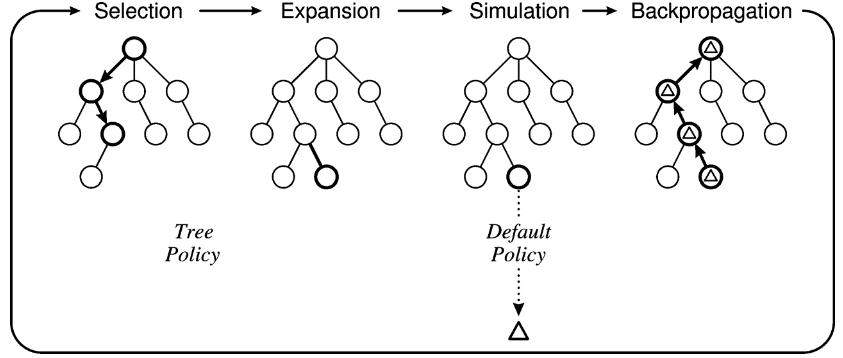
\includegraphics[width=0.7\columnwidth]{Background/MCTS_approach.png}
      \caption[MCTS approach]
      {One MCTS iteration \cite{browne_survey_2012}}
      \label{fig:mcts_approach}
\end{figure}

The algorithm consists of four phases, as illustrated in Figure \ref{fig:mcts_approach}  \cite{browne_survey_2012}. These phases are repeated for a predefined number of iterations or until a computational budget (such as time or memory) is reached. The phases are as follows:

\begin{enumerate}
	\item \textbf{Selection:} The tree is traversed from the root node until it finds a node that is not completely expanded, i.e., a non-terminal node with unvisited children. The selection is guided by a policy that balances exploration and exploitation. Typically, the policy used is \ac{uct}, which selects nodes that maximize formula \ref{uct_formula}.
	 
	\begin{equation}
	UCT = \overline{X_i} + 2C\sqrt{\frac{2\ln{n}}{n_i}},\label{uct_formula}
	\end{equation} where \(\overline{X_i}\) is the total reward of all playouts through this state by the number of visits, \(C\) is a constant greater than zero (typically \sqrt{2}), \(n_i\) is the number of visits of child node \(i\), and \(n\) is the number of visits of the parent node.
    \item \textbf{Expansion:} One or more child nodes are added to the node previously reached in the selection phase.
    \item \textbf{Simulation:} From the newly added node(s), a simulation is performed according to a default policy, which may include random moves until a terminal node is reached.
    \item \textbf{Backpropagation:} The simulation result is then propagated back through the traversed nodes, where the number of visits and the average reward for each node are updated until it reaches the root.
\end{enumerate}

\section{Local Search}

Local search is an optimization technique that iteratively improves a solution within a given search space by making small changes and retaining those that yield better results. It is effective for large-scale problems where the search is computationally expensive or unfeasible. Popular local search algorithms include Hill Climbing, Simulated Annealing, Tabu Search, and Genetic Algorithms. While local search algorithms are powerful, they can sometimes get stuck and fail to find the global best solution. Techniques such as simulated annealing help escape local optima and explore a broader range of solutions.

\subsection{Hill Climbing}

\ac{hc} is a local search optimization algorithm that begins with an initial solution, which can be randomly generated or specifically chosen depending on the problem. From this starting point, \ac{hc} evaluates neighbouring solutions, which are generated by making small modifications to the current solution. If a neighbouring solution is found to be better than the current one, the algorithm moves to that new solution. The algorithm finishes when there is no better neighbouring solution that offers an improvement over the current one, indicating that a local optimum has been attained. 

While \ac{hc} is effective and easy to implement, it has limitations.The algorithm can get stuck in:

\begin{itemize}
\item \textbf{Local optimum:} A solution state that is better than its neighbours but not necessarily the global optimum, i.e., the best possible solution in the entire search space, restricting further improvement.
\item \textbf{Plateaus:} Mostly flat regions in the search space where neighbouring solutions have the same value, making it challenging for the algorithm to determine a direction of improvement.
\item \textbf{Ridges:} A region in the search space where moving in all directions appears to lead downhill, and reaching a better solution often requires a sequence of non-improving moves, which \ac{hc} does not explore.
\end{itemize}

To address these issues, variations of the algorithm have been developed:

\begin{itemize}
\item \textbf{Simple Hill-Climbing:} Evaluates one neighbour at a time and moves to the first improvement found, making it efficient but susceptible to local maxima.
\item \textbf{Steepest-Ascent Hill-Climbing:} Evaluates all neighbours of the current state and chooses the best among them. This algorithm is a variation of the simple hill-climbing algorithm but takes more time.
\item \textbf{Stochastic Hill-Climbing}: Randomly selects a neighbour, without evaluation, and moves to it if it improves the solution. This approach is less commonly used than the other two.
\end{itemize}

\section{Previous Work}

\begin{figure}
      \centering
      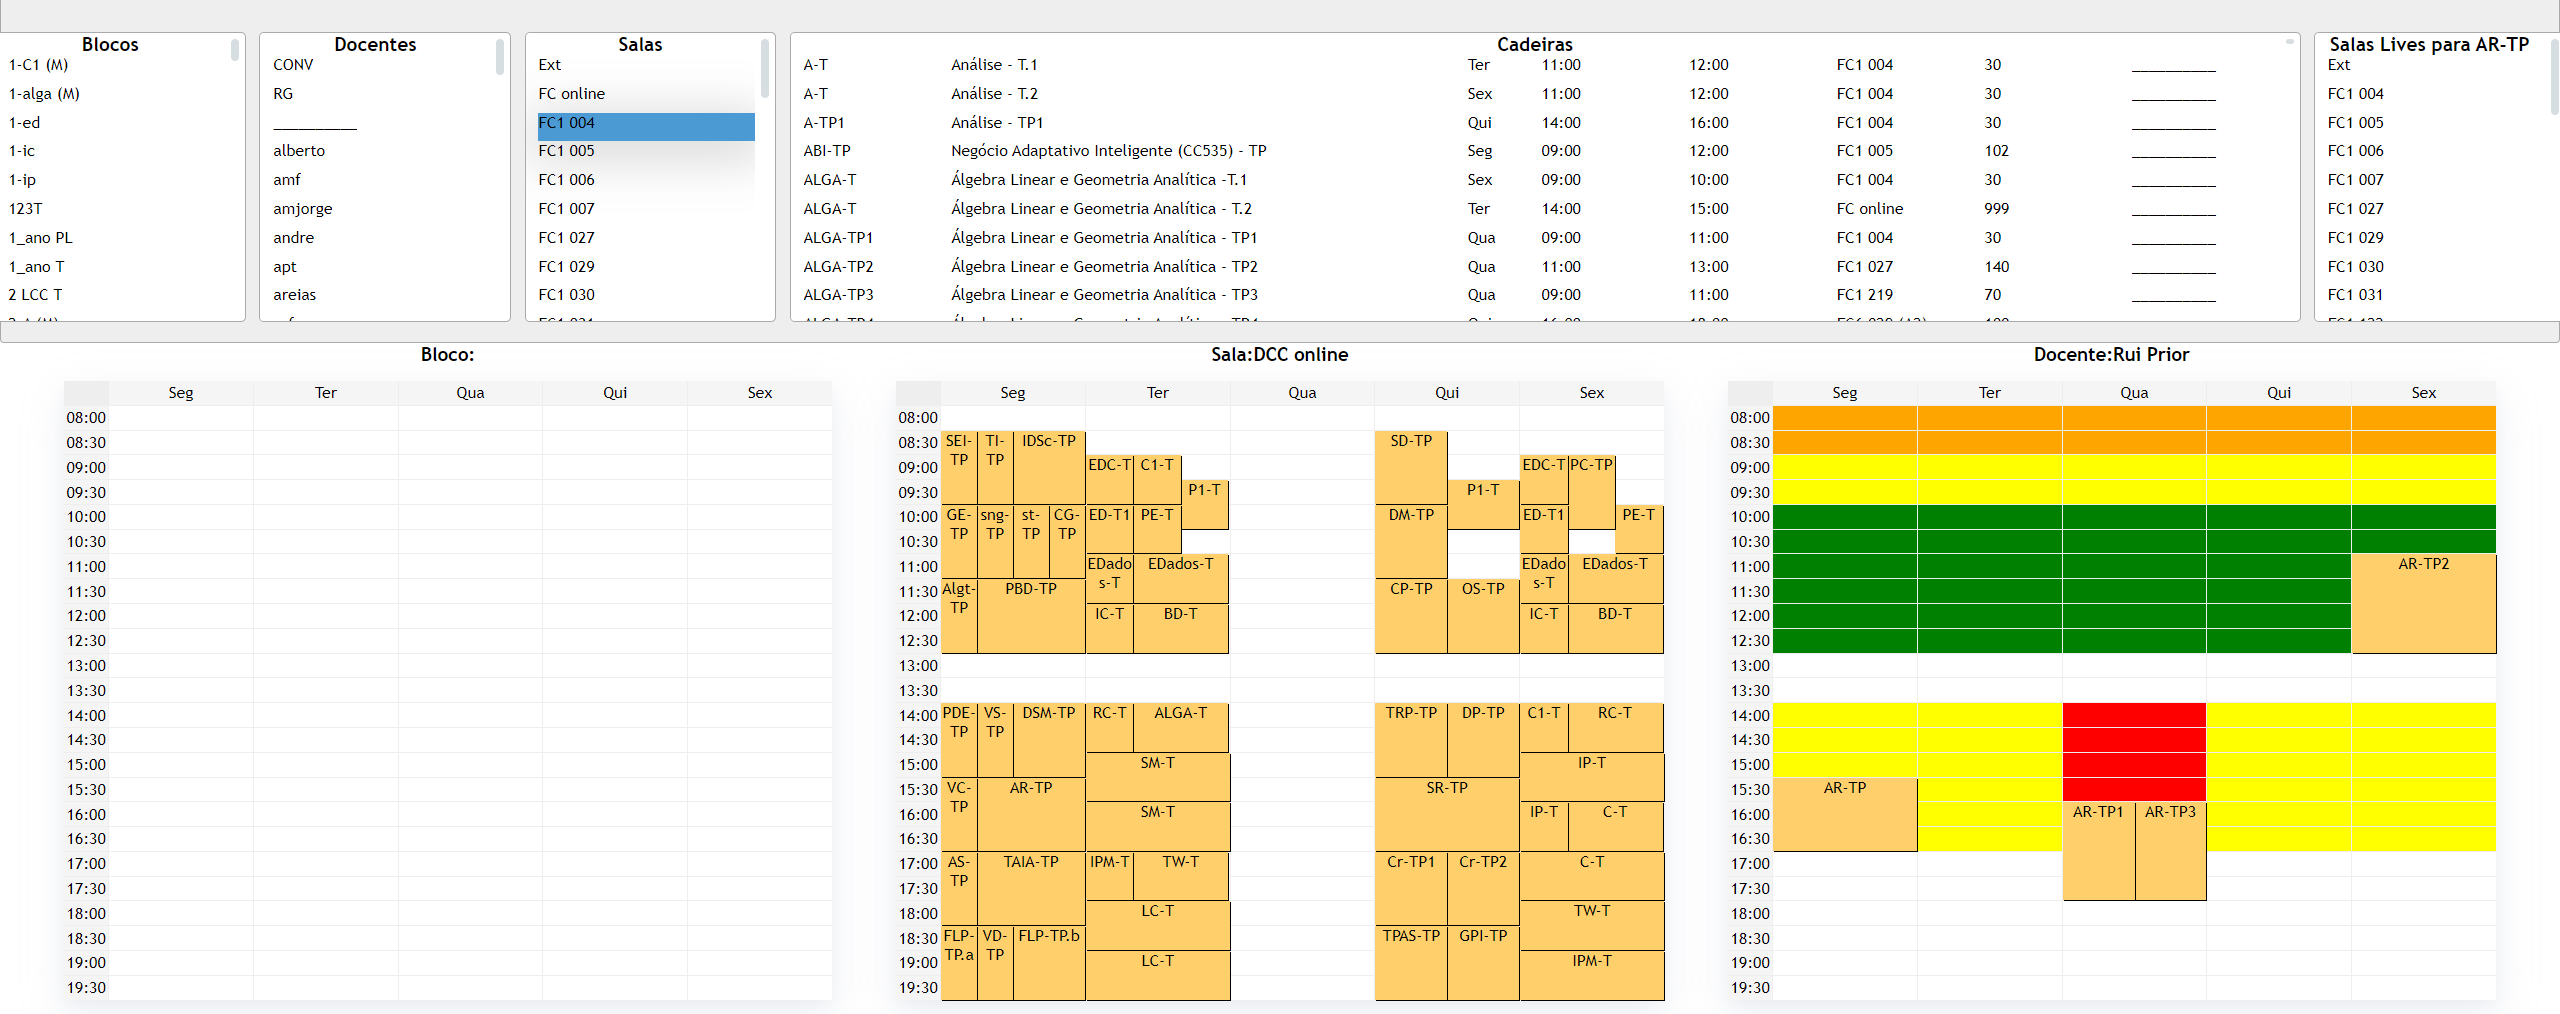
\includegraphics[width=1.0\columnwidth]{Background/previous_work.png}
      \caption[Previous work interface]
      {Previous work interface}
      \label{fig:previous_work_interface}
\end{figure}

\begin{figure}
      \centering
      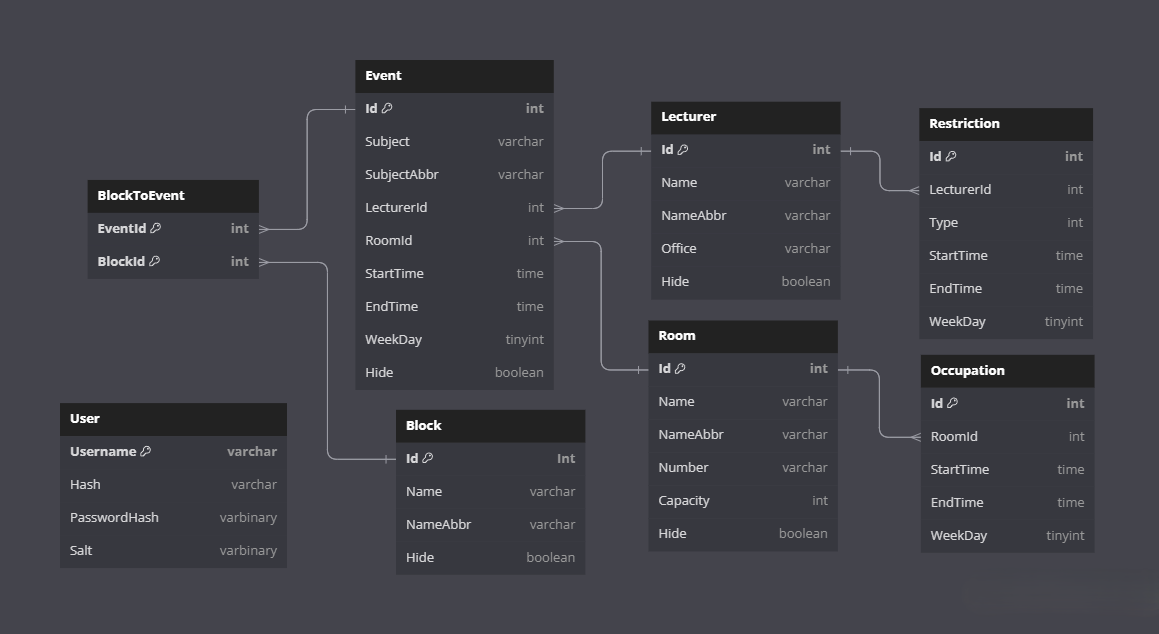
\includegraphics[width=1.0\columnwidth]{Background/uml.png}
      \caption[Previous work UML]
      {Previous work UML}
      \label{fig:previous_work_uml}
\end{figure}

A previous project\footnote{\textbf{Front-end:} \url{https://github.com/luismdsleite/schedule} \textbf{Back-end:} \url{https://github.com/luismdsleite/schedule-backend/tree/main}} developed a timetabling visualization tool using Flask and reactive programming principles with the Elm language. Flask facilitated data management and communication between the front-end and the database (Figure \ref{fig:previous_work_uml}), ensuring that timetable updates were efficiently processed and displayed. 

This tool allow users to manually construct and modify schedules while providing a responsive interface (Figure \ref{fig:previous_work_interface}). However, despite its usability, the tool has some limitations that this dissertation attempts to address:

\begin{itemize}
\item \textbf{No conflict detection support:} Users had to manually check for conflicts, increasing the risk of errors.
\item \textbf{Lack of automated guidance:} It did not provide recommendations or suggestions to help users make optimal scheduling decisions.
\item \textbf{No quality assessment:} The system lacked mechanisms to evaluate the quality of a given timetable.
\end{itemize}

%\subsection{Reactive Programming}

%\subsubsection{Elm}



\pretocmd{\chapter}{\glsresetall}{}{}

% Related

% Main chapter title
%\chapter[toc version]{doc version}
\chapter{Related Work}

% Short version of the title for the header
%\chaptermark{version for header}

% Chapter Label
% For referencing this chapter elsewhere, use \ref{ChapterTemplate}
\label{Related Work}

The literature on the\ac{ucttp} is vast, so this chapter will cover various approaches to address this problem, mostly based on surveys.

According to Lewis' survey \cite{lewis_survey_2008}, algorithms can be divided into three categories:

\begin{itemize}
	\item \textbf{One-Stage} algorithms use a weighted sum function of constraints to identify solutions that satisfy both hard and soft constraints at the same time;
	\item \textbf{Multi-Stage} algorithms aim to optimize soft constraints while ensuring feasibility;
	\item \textbf{Multi-stage with relaxation} is divided into multiple stages, with some constraints being relaxed while satisfying others.
\end{itemize}

Other surveys, such as Abdipoor et al.\ \cite{abdipoor_meta-heuristic_2023}, categorized\ac{ucttp} into five groups: operational research, metaheuristics, hyperheuristics, multi-objective, and hybrid approaches.

\section{Operational Research (OR)}

Operational Research (OR) techniques provide mathematically rigorous solutions. Despite their complexity, these methods are simple to implement and can be considered if time and memory constraints are not a concern \cite{babaei_survey_2015}. However, if time is limited, the other types of approaches provide better quality results. 

As Babaei et al.\ and Chen et al.\ detailed in their surveys \cite{babaei_survey_2015,chen_survey_2021}, OR includes Graph Coloring (GC), Integer and Linear Programming (IP/LP) and Constraint Satisfaction(s) Programming (CSPs) based techniques.

\section{Metaheuristics}

Metaheuristics \textit{provide "acceptable" solutions in a reasonable time for solving hard and complex problems} \cite{talbi2009metaheuristics}. 

Metaheuristics are similarly defined by Du et al.\ as \textit{a class of intelligent self-learning algorithms for finding near-optimum solutions to hard optimization problems} \cite{du2016search}.

Metaheuristics, while not guaranteeing global optimality, have become one of the most used solution strategy for\ac{ucttp} and can be classified into two categories: Single solution-based and Population-based.

\subsection{Single Solution-Based}

Single solution-based metaheuristics, also known as local search algorithms, focus on modifying a single solution throughout the search in order to improve that solution. 

This metaheuristic approach includes algorithms such as\ac{hc},\ac{sa},\ac{ts}, and Iterated Local Search (ILS).\ac{sa} is perhaps the most effective single solution-based metaheuristic, particularly in benchmark datasets, but\ac{ts} has also been shown to be successful in minimizing hard constraints \cite{abdipoor_meta-heuristic_2023}.

\subsection{Population-Based}

Population-based meta-heuristics iteratively improve a population of solutions by generating a new population based on the selection, recombination and/or mutation of individuals in the current population. This method can be subdivided into Evolutionary Algorithms, such as Genetic Algorithms, and Swarm Intelligence, such as Ant Colony Optimization \cite{abdipoor_meta-heuristic_2023,du2016search}.

Population-based metaheuristics, as opposed to single-solution-based metaheuristics, are more focused on exploration rather than exploitation \cite{talbi2009metaheuristics,du2016search}. Despite promising results on real-world datasets, population-based approaches were rarely applied to benchmark datasets and performed poorly in\ac{itc} competitions compared to single solution-based methods \cite{abdipoor_meta-heuristic_2023}.

%\subsubsection{Hybrid}

\section{Hyperheuristics}

Heuristic methods have been highly effective in solving a wide range of problems. However, their application to new problems is often challenging due to the vast number of parameter tuning and the lack of clear guidance \cite{hyper_heuristics_survey}. To address this problem, hyperheuristics aim to generalize methods by selecting or combining the most suitable heuristic(s) for a specific problem, rather than explicitly solving the problem.

Hyperheuristic approaches are less common, possibly due to their performance \cite{chen_survey_2021}.

\section{Multi-Objective Optimization}\label{sec:mo}

Multi-objective or multi-criteria approaches aim to optimize multiple conflicting objectives simultaneously. These methods are frequently used to find the optimal Pareto front, which is a set of compromise optimal solutions such that one cannot improve one objective without deteriorating the other. However, the disadvantage of this approach lies in the execution effort \cite{chen_survey_2021}. Several multi-criteria algorithms can also be included in other categories, such as metaheuristics.

\section{Hybrid Approaches}

Hybrid approaches mix algorithms from two or more of the previously mentioned types of approaches.

Hybrid approaches can indeed be divided into two main categories \cite{abdipoor_meta-heuristic_2023}:

\begin{itemize}
\item \textbf{Collaborative hybrids:} Involve running different algorithms sequentially, intertwined, or in parallel, sharing information without structural integration. This collaboration enables each component to focus on its area of the problem, with occasional communication guiding the overall search process.

\item \textbf{Integrative hybrids:} Integrate components of different algorithms into a single framework, creating a cohesive and interdependent method.

\end{itemize}

%Hybridization of local search and population-based approaches (also known as the Memetic Algorithm (MA))

In particular, Tomáš Müller, winner of the\ac{itc-2007} tracks 1 and 3, developed a collaborative hybrid approach\footnote{\url{https://github.com/tomas-muller/cpsolver-itc2007}} for all three tracks \cite{muller_itc2007}, finding feasible solutions for all instances of tracks 1 and 3 and most instances of track 2. 

The algorithms used included Iterative Forward Search (IFS),\ac{hc}, Great Deluge (GD), and optionally\ac{sa}. During the construction phase, IFS is employed to find a complete solution, followed by\ac{hc} to find the local optimum. When a solution cannot be improved further using\ac{hc}, GD is used to iteratively decrease, based on a cooling rate, a bound that is imposed on the value of the current solution. Optionally,\ac{sa} can be used when the bound reaches its lower limit.

The solver's techniques have been integrated into the UniTime\footnote{\url{https://www.unitime.org/}} system, which is widely used for scheduling in academic institutions. Furthermore, the principles behind Müller's hybrid methodology are still relevant in modern optimization methods.

While Müller's approach was highly successful in 2007, subsequent research has revealed that other methods may outperform it in some instances. However, it remains a benchmark against which new approaches are often compared.

\section{Monte Carlo Tree Search}

\ac{mcts} application to \acp{cop} remains relatively unexplored. In the context of\ac{ucttp}, Goh's investigation \cite{goh_MCTS} is the only known study that explores the potential of\ac{mcts} in solving the\ac{pe-ctt}. 

Goh's investigation employs a two-stage approach, first utilizing\ac{mcts} to find initial feasible solutions and then applying local search techniques to enhance the quality of these solutions.

The research introduces several enhancements to the standard\ac{mcts} algorithm, including heuristic-based simulations and tree pruning techniques, which improved the\ac{mcts} performance and effectiveness. The study also provides a comprehensive comparison of\ac{mcts} against traditional methods such as Graph Coloring heuristic and\ac{ts}, with\ac{ts} emerging as the most effective method.

One major limitation of\ac{mcts} for timetabling is, as highlighted by Goh, its rigorous decision-making process. Events are assigned sequentially and cannot be reassigned, limiting the algorithm's flexibility. In contrast, local search methods, such as\ac{ts}, allow dynamic reassignment, enabling a more efficient exploration of the search space. Furthermore, the tree-based structure of\ac{mcts} restricts its hybridization with local search techniques, which have proven essential in achieving significant results in other learning-based algorithms. Another drawback of\ac{mcts} is its high computational cost, making it less effective under the strict time constraints imposed by timetabling problems.

This dissertation aims to demonstrate that, despite its limitations,\ac{mcts} still holds potential for timetabling problems with the appropriate modifications and hybridization. 

\section{Summary}

We analyzed various surveys \cite{lewis_survey_2008,abdipoor_meta-heuristic_2023,babaei_survey_2015,chen_survey_2021} and categorized\ac{ucttp} approaches based on their problem-solving strategies:

\begin{itemize}
\item Metaheuristics emerged as one of the most promising, particularly single-solution-based algorithms like\ac{sa} and\ac{ts}.
\item Hybrid approaches, like Müller’s\ac{itc-2007} approach \cite{muller_itc2007}, were also shown to be effective.
\item Operational research methods are simple to implement but are often outperformed due to scalability limitations.
\item Hyperheuristics, while still emerging, aim to generalize methods by dynamically selecting among heuristics.
\item Multi-objective methods optimize multiple conflicting objectives simultaneously, but they are computationally expensive.
\item Goh \cite{goh_MCTS} study on the\ac{pe-ctt} found that\ac{ts} outperformed\ac{mcts}, despite improvements to the standard\ac{mcts} algorithm.
\item\ac{mcts} and its hybridization remain unexplored in the context of\ac{cb-ctt}, making this the novel contribution of our work.
\end{itemize}























% Development

% Main chapter title
%\chapter[toc version]{doc version}
\chapter{Development}

% Short version of the title for the header
%\chaptermark{version for header}

% Chapter Label
% For referencing this chapter elsewhere, use \ref{ChapterTemplate}
\label{Development}

This chapter describes the development of the timetable system, formulating the problem, discussing the implementation of the \ac{mcts} and \ac{hc} hybrid approach, detailing the design choices, algorithmic improvements and integration efforts made throughout the project.

\section{Problem Formulation}

The entities in the problem are listed below:

\begin{itemize}
	\item \textbf{Periods, \(P = \{P_0, P_1, ..., P_|_P_|_-_1\}\):} Days are divided into fixed timeslots, with periods consisting of a day and a timeslot.

		%\unsure[inline]{In the previous work, there is no periods. There are weekdays, a start time and an end time. For now, in the current approach, an event is only associated with a period of one hour and without any link to previous work. If I implement this concept to previous work, an event should be assigned to one or more half-hour periods.}

	\item \textbf{Rooms, \(R = \{R_0, R_1, ..., R_|_R_|_-_1\}\):} Each room has a capacity and a type.
		\begin{itemize}
			%\item Occupation (the room may be utilized for non-teaching reasons, such as exams) (TODO)
			\item Capacity (number of seats)
			%\item Type (TODO)
		\end{itemize}

	\item \textbf{Lecturers, \(L = \{L_0, L_1, ..., L_|_L_|_-_1\}\):} 
		\begin{itemize}
			%\item Office
			\item Availability
			%\item Restriction (availability and TODO: preferences for periods)
		\end{itemize}

	\item \textbf{Events, \(E = \{E_0, E_1, ..., E_|_E_|_-_1\}\):} Represent the events to be scheduled (usually a lecture). Each event has associated attributes:
%		\begin{multicols}{2}
%		\textbf{Previous work:}
%		\begin{itemize}
%			\item Start and end time
%			\item Weekday
%			\item Duration
%			\item Lecturer
%			\item Room
%		\end{itemize}
%		\columnbreak
%		\textbf{TODO: adicionar ao trabalho anterior?}
		\begin{itemize}
        		\item Capacity (number of students)
        		\item Number of lectures
        		\item Minimum working days (days over which the events of the same course should be spread)
        		\item Available periods
        		\item Priority
        		\item Lecturer
        		\item Period (day, timeslot)
 			\item Room
		\end{itemize}
%		\end{multicols} 

	\item \textbf{Blocks, \(B = \{B_0, B_1, ..., B_|_B_|_-_1\}\):} A block may represent a group of related events. Usually represents all events from the same curriculum, which is a set of courses in a study program.
\end{itemize}

\subsection{Constraints}

There are several hard and soft constraints that affect the creation of \ac{fcup} timetables. The following hard and soft constraints were selected, drawing inspiration from those of \ac{itc-2007}:

\textbf{Hard constraints:}

\begin{itemize}
	\item \textbf{H1:} Events belonging to the same course must be scheduled and must be assigned to distinct periods.
	\item \textbf{H2:} Two events can be scheduled in the same room, but only if they are in different periods.
	\item \textbf{H3:} Events of the same curricula, or taught by the same lecturer, must be scheduled in different periods.
	\item \textbf{H4:} If a lecturer is unavailable in a given period, then no events can be taught by this lecturer in that period.
%	\item \textbf{TODO H5:} If a room is unavailable in a given period, then no events can be scheduled in that period.
%	\item \textbf{TODO H6:} Lecturers and students must have a free lunch period.
\end{itemize}

\textbf{Soft constraints:}

\begin{itemize}
	\item \textbf{S1:} Events of the same course should be spread into the given minimum number of days.
	\item \textbf{S2:} Events belonging to the same curriculum should be in consecutive periods.
	\item \textbf{S3:} The capacity of the room should be higher or equal than the capacity of the event.
	\item \textbf{S4:} All events of a course should be given in the same room.
\end{itemize}

The problem is defined as a maximization problem, with the algorithm attempting to minimize soft constraint violations while strictly adhering to hard constraints.

\section{Monte Carlo Tree Search}

%This section describes the key algorithmic components of the system, particularly the hybrid \ac{mcts} with \ac{hc} approach.

%(...)

\subsection{Search Space}

The search space, \(S\),  for this problem is large as it involves a product of all possible event-period-room combinations: \[S = E \cdot P  \cdot R,\] where \(E\) is the set of events, \(P\) is the set of periods (day, timeslot), and \(R\) is the set of rooms.

To reduce the search space, unavailable periods and unavailable rooms for a chosen period are discarded immediately in the \ac{mcts} \(expansion\) phase.

\subsection{\ac{mcts} Tree}

\begin{figure}
      \centering
      \includegraphics[width=0.7\columnwidth]{Development/MCTS_tree.jpg}
      \caption[MCTS tree]
      {MCTS tree}
      \label{fig:mcts_tree}
\end{figure}

Figure \ref{fig:mcts_tree} illustrates the basic structure of the \ac{mcts} tree. The root represents the initial state, where no events have been assigned. The first level corresponds to assigning the first event, \(E_0\), to various \(P\) and \(R\). Each child node represents a specific assignment (\((E_0,P_0,R_0),...,(E_0,P_|_P_|_-_1,R_|_R_|_-_1)\)). Subsequent levels correspond to the sequential assignment of events \(E_1, E_2, ..., E_|_E_|_-_1\).

\subsubsection{Tree Nodes}

A node is composed of the following attributes:

\begin{itemize}
\item A \textbf{path} is a dictionary that represents the sequence of actions leading to a node. The root is the only node that has an empty path.

\item A \textbf{parent} is a reference to the parent node, allowing the tree structure to be navigated upwards. The root is the only node that does not have a parent.

\item \textbf{Children} is initialized as an empty list at first but will later hold references to the node's child nodes. 

\item The \textbf{expansion limit} specifies the maximum number of children that a node can have, which helps control the expansion process. It is estimated based on the number of available rooms per period for the next event. A value of zero indicates that the node cannot be expanded further.

\item \textbf{Visits} is initialized to 0, tracking the number of times a node has been visited.

\item The \textbf{hard and soft scores} are both initialized to 0, representing the cumulative hard and soft scores for a node, which are used to evaluate the quality of the node's state.

\item The \textbf{best hard and soft penalty results} are initialized to negative infinity, representing the best hard and soft penalty results encountered for a node. These attributes will be updated during the algorithm as better results are found. 
\end{itemize}

\subsection{Events Allocation}

Events are sorted in advance so that the most difficult event to place is placed first in the tree. The priority of an event (Formula \ref{priority}) is calculated based on:

\begin{itemize}
\item The difference between the number of lectures and minimum working days to prioritize events with more lectures spread over fewer days;
\item The number of available periods, as having more available periods indicates fewer scheduling restrictions;
\item The capacity of an event, which implies that events with greater capacity have higher priority;
\item The number of curricula in which the event is, as events that appear in more curricula are more difficult to allocate.
\end{itemize}

If two or more events have the same priority score, they are ordered randomly.

\begin{equation}
  \begin{aligned}
	Priority = (\#lectures - \#min\_working\_days) \cdot 4 \\
	           - \#available\_periods \cdot 3 \\
	          + capacity \cdot 2 \\
	          + \#blocks\label{priority}
  \end{aligned}
\end{equation}

%I have tried other priority formulas...

\subsection{Periods and Rooms Allocation}

Initially, our approach to allocating periods and rooms in the \ac{mcts} tree followed a structured sequence. This method aimed to explore all possible (period, room) combinations based on the number of children of the current node being expanded. However, as we progressed, this approach started to fail when the availability of rooms varied across different periods. A refined approach was then developed to address these limitations more robustly.

\subsubsection{Initial Periods and Rooms Allocation Approach}

In the initial approach, each event assignment generated in the \ac{mcts} tree follows a structured sequence for period and room allocation. 
Let:
\begin{itemize}
\item \(n\) be the number of children of the current node being expanded;
\item \(AP\) the number of available periods;
\item \(AR\) the number of available rooms. 
\end{itemize}

The assignment is determined as follows:

\begin{itemize}
	\item The period index was selected using: 
		\begin{equation}
		n \mod AP\label{period_allocation}
		\end{equation}
	
	\item The room index was selected using:
		\begin{equation}
		\frac{n}{AP} \mod AR\label{room_allocation}
		\end{equation}
\end{itemize}

This resulted in a deterministic exploration order. For instance, if \(AP = 3\) and \(AR = 2\), the assignment would be:
\[
\begin{aligned}
n = 0 &\Rightarrow P_0, R_0 \\
n = 1 &\Rightarrow P_1, R_0 \\
n = 2 &\Rightarrow P_2, R_0 \\
n = 3 &\Rightarrow P_0, R_1 \\
n = 4 &\Rightarrow P_1, R_1 \\
n = 5 &\Rightarrow P_2, R_1 \\
\end{aligned}
\]

This approach assumes that the number of children will always perfectly expand all (period, room) combinations, but it fails when the search space is reduced, resulting in different periods having different available rooms.

Consider the following scenario:
\begin{itemize}
\item Available Periods = \([(0,1), (3,2)]\)
\item Rooms at (0,1) = \(['C', 'D', 'E', 'F', 'G']\) (5 rooms)
\item Rooms at (3,2) = \(['B']\) (1 room)
\end{itemize}

Here, \(AP = 2\), but the number of available rooms (\(AR\)) depends on the period. The expansion limit is 6, thus we compute assignments from \(n = 0\) to \(n = 5\):

\[
\begin{aligned}
n = 0: &\quad P_0 = (0,1),\quad R_0 = 'C' \quad &\text{(Valid)} \\
n = 1: &\quad P_1 = (3,2),\quad R_0 = 'B' \quad &\text{(Valid)} \\
n = 2: &\quad P_0 = (0,1),\quad R_1 = 'D' \quad &\text{(Valid)} \\
n = 3: &\quad P_1 = (3,2),\quad R_0 = 'B' \quad &\text{(Invalid: Duplicate)} \\
n = 4: &\quad P_0 = (0,1),\quad R_2 = 'E' \quad &\text{(Valid)} \\
n = 5: &\quad P_1 = (3,2),\quad R_1 = 'B' \quad &\text{(Invalid: Duplicate)} \\
\end{aligned}
\]

Because room availability is period-specific, the formula produces duplicate assignments when \(AR\) is not consistent across all periods.

\subsubsection{Final Periods and Rooms Allocation Approach}

To overcome these limitations, instead of computing the (period, room) combinations via index math, we pre-compute all valid combinations once. This method produces a flat list of unique, valid assignments, and expansion always proceeds without duplication.

Moreover, periods that are less frequently available across all events are given higher priority. In this way, the algorithm reduces the risk of future conflicts, guiding the tree toward more constrained decisions early. For each period, available rooms are also sorted by how closely their capacity matches the event’s requirements, minimizing wasted space and increasing flexibility in room usage.

\subsection{Methodology}

The \ac{mcts} algorithm consists of four phases: \(selection\), \(expansion\), \(simulation\), and \(backpropagation\). Each phase plays a critical role in exploring the search space and updating the tree structure with the simulation outcomes. Figure \ref{fig:mcts_steps} provides a high-level overview of these four phases in the \ac{mcts} process.

\begin{figure}[H]
      \centering
      \includegraphics[width=1.1\columnwidth]{Development/MCTS_Steps.jpg}
      \caption[MCTS steps]
      {MCTS steps}
      \label{fig:mcts_steps}
\end{figure}

\subsubsection{Selection}

The \(selection\) phase (Algorithm \ref{selection}) begins at the root and traverses the tree by iteratively selecting the best child nodes until a terminal (leaf) node is reached. A node is considered terminal if either it cannot be expanded further (i.e., its expansion limit is zero) or if it has reached the maximum depth (i.e., all the events have been assigned). Conversely, a node is deemed fully expanded if either its expansion limit is zero or if the number of its children equals its expansion limit. When the traversal encounters a node that is not fully expanded, the process stops, and that node is selected for further expansion.

The best child node (Algorithm \ref{best_child}) is determined by applying the \ac{uct} formula (\ref{uct_formula}). However, as the problem has two goals, maximizing the hard constraints first and then the soft constraints, the \ac{uct} formula was applied differently. Initially, the algorithm computes the weights for each child node using the hard score. Among the children with the highest hard score, the weights are recalculated based on the soft score. The child node with the highest weight in this second calculation is selected as the best child. However, if all of a node's children have reached their expansion limit, the algorithm backtracks: if the current node has a parent, the current node expansion limit is set to zero, and it moves up to the parent. Reaching the root indicates that the entire tree is fully expanded.

\begin{algorithm}
\caption{Selection}\label{selection}
\begin{algorithmic}[1]
\Procedure{SELECTION}{}
    \State current\_node $\gets$ root
    \While{not current\_node.\textit{is\_terminal\_node}(\textit{len}(events))}
        \If{not current\_node.\textit{is\_fully\_expanded}()}
            \State \textbf{break}
        \EndIf
        \State unflagged\_children $\gets$ [child \textbf{for each} child \textbf{in} current\_node.children \textbf{if} child \textbf{and} child.expansion\_limit $\neq$ 0]
        \If{unflagged\_children is empty}
            \If{current\_node.parent exists}
                \State current\_node.expansion\_limit $\gets 0$
                \State current\_node $\gets$ current\_node.parent
            \Else
                \State \Return False
            \EndIf
        \Else
            \State current\_node $\gets$ current\_node.\textit{best\_child}(unflagged\_children)
        \EndIf
    \EndWhile
    \State self.current\_node $\gets$ current\_node
    \State \Return True
\EndProcedure
\end{algorithmic}
\end{algorithm}

\begin{algorithm}
\caption{Best Child}\label{best_child}
\begin{algorithmic}[1]
\Function{BEST\_CHILD}{unflagged\_children, c\_param = 1.4}
    \State choices\_weights $\gets$ [$\frac{child.score\_hard}{child.visits} $+$ c\_param $\cdot \sqrt{\frac{2\ln(self.visits)}{child.visits}}$ \textbf{for each} child \textbf{in} unflagged\_children]
    \\
    \State max\_weight $\gets$ \textit{max}(choices\_weights)
    \State best\_children $\gets$ [unflagged\_children[i] \textbf{for each} i, weight \textbf{in} \textit{enumerate}(choices\_weights) \textbf{if} weight = max\_weight]
    \\
    \State choices\_weights $\gets$ [$\frac{child.score\_soft}{child.visits} $+$ c\_param $\cdot \sqrt{\frac{2\ln(self.visits)}{child.visits}}$ \textbf{for each} child \textbf{in} best\_children]
    \\
    \State \Return best\_children[\textit{index\_of}(\textit{max}(choices\_weights))]
\EndFunction
\end{algorithmic}
\end{algorithm}

\subsubsection{Expansion}

The \(expansion\) phase (Algorithm \ref{expansion}) is responsible for expanding the node previously selected by assigning the next event to a valid (period, room) combination and creating a corresponding child node.

The next event to schedule is determined by the depth of the current node. For the selected event, the algorithm gathers the available (weekday, timeslot) combinations and filters suitable rooms for each period (Algorithm \ref{find_available_rooms}), based on the event’s capacity requirements and current room occupation.

A list of valid (period, room) combinations is generated. If no such combinations exist or the node has already been expanded for all possibilities, expansion is terminated, and the node is marked as fully expanded.  

A combination is selected based on the number of already-expanded children. A new path is constructed by assigning the selected period and room to the event.

Before proceeding, the algorithm evaluates the partial timetable (i.e., the new path) against a global hard penalty threshold. If the new assignment violates hard constraints resulting in a penalty below the threshold, a null child is added to indicate that the expansion stopped for that branch. This pruning was introduced as a mechanism to eliminate paths in the tree that violate hard constraints, thus focusing computational effort on promising and feasible solutions.

If the expansion continues, the algorithm estimates the number of valid (period, room) combinations for the next event. This value is stored as the child’s expansion\_limit to guide future branching.

Finally, a new child node is created with the updated path and expansion limit. This new node is added to the tree, and the current node is updated to this newly created node.

\begin{algorithm}
\caption{Expansion}\label{expansion}
\begin{algorithmic}[1]
\Function{EXPANSION}{}
    \State event $\gets$ events[current\_node.\textit{depth}()]
    \State available\_periods $\gets$ event["Available\_Periods"]
    \\
    \If{available\_periods is empty}
        \State current\_node.expansion\_limit $\gets$ 0
        \State \Return False
    \EndIf
    \\
    \State rooms\_by\_period $\gets$ \textit{find\_available\_rooms}()
    \State period\_room\_combinations $\gets$ [(weekday, timeslot, room) \textbf{for} (weekday, timeslot), rooms in room\_by\_period.\textit{items()}]
    \\
    \If{period\_room\_combinations is empty \textbf{or} current\_node is fully expanded}
        \State current\_node.expansion\_limit $\gets$ 0
        \State \Return False
    \EndIf
    \\
    \State new\_weekday, new\_timeslot, new\_room $\gets$ period\_room\_combinations[len(current\_node.children)]
    \State new\_path $\gets$ \textit{copy}(current\_node.path)
    \State new\_path[event["Id"]] $\gets$ \{**event, "RoomId": new\_room, "WeekDay": new\_weekday, "Timeslot": new\_timeslot\}
    \\
    \State new\_expansion\_limit $\gets$  = \textit{calculate\_expansion\_limit}(new\_path)
    \State \textbf{if} new\_expansion\_limit is None: \Return False
    \\
    \State child\_node $\gets$ MCTSNode(expansion\_limit = expansion\_limit, parent = current\_node, path = new\_path)
    \State current\_node.children.\textit{append}(child\_node)
    \State current\_node $\gets$ child\_node
    \State \Return True
\EndFunction
\end{algorithmic}
\end{algorithm}

\begin{algorithm}
\caption{Find Available Rooms}\label{find_available_rooms}
\begin{algorithmic}[1]
\Function{FIND\_AVAILABLE\_ROOMS}{event\_capacity, rooms, events, available\_periods}
    \State period\_room\_availability $\gets$ \{period: \textit{set}(rooms.keys()) \textbf{for each} period \textbf{in} available\_periods\}
    \For{\textbf{each} other\_event \textbf{in} events}
        \State occupied\_period $\gets$ (other\_event["WeekDay"], other\_event["Timeslot"])
        \If{occupied\_period \textbf{in} period\_room\_availability}
            \State period\_room\_availability[occupied\_period].\textit{discard}(other\_event["RoomId"])
        \EndIf
    \EndFor
    \\
    \State suitable\_rooms $\gets$ \{room\_id \textbf{for each} room\_id, room \textbf{in} rooms.items() \textbf{if} room["Capacity"] $\geq$ event\_capacity\}
    \\
    \For{\textbf{each} period \textbf{in} available\_periods}
        \If{period\_room\_availability[period] is not empty}
            \State intersected $\gets$ period\_room\_availability[period] $\cap$ suitable\_rooms
            \If{intersected is not empty}
                \State sorted\_rooms $\gets$ \textit{sort}(intersected, by (room["Capacity"] - event\_capacity))
            \Else
                \State sorted\_rooms $\gets$ \textit{sort}(period\_room\_availability[period], by $|$room["Capacity"] - event\_capacity$|$)
            \EndIf
            \State period\_room\_availability[period] $\gets$ sorted\_rooms
        \EndIf
    \EndFor
    \\
    \State \Return period\_room\_availability
\EndFunction
\end{algorithmic}
\end{algorithm}

\subsubsection{Simulation}

The \(simulation\) phase estimates the value of multiple actions, in this case, distinct event allocations, which will guide the selection and expansion steps in future iterations. 

A random event allocation approach was initially explored but produced suboptimal results. Therefore, a more structured method was implemented.

The \(simulation\) function (Appendix \ref{AppendixA} Algorithm \ref{simulation}) starts by creating a copy of the current node's path, which contains the events already scheduled. It then identifies the remaining events, i.e., events that have not been assigned yet. These remaining events are sorted based on two criteria:
\begin{enumerate}
\item Whether they were previously unassigned in prior simulations, to prioritize harder-to-schedule events.
\item Their priority, ensuring that more critical events are allocated first.
\end{enumerate}

For each unvisited event, the best available period and room combination is sought. The approach iterates through all the available periods and rooms, calculating the hard and soft penalties for each combination. During the calculation of the soft penalty, the importance of compactness (i.e., minimizing the time between related events) is adjusted, with a higher weight applied as the algorithm progresses.The combination with no hard penalties and the lowest soft penalty is selected as the best option. If multiple optimal choices exist, one is randomly selected. The event is then updated with the selected room, weekday, and timeslot. If no valid allocation is found, the event will have higher priority in the next simulation.

After scheduling all events, the simulation result is calculated, and the best and worst penalty scores are then updated based on these results. If a new best result is found, the timetable is saved to a file. If a new best result is found and the hard penalty is zero, indicating a feasible solution, the \ac{hc} algorithm (section \ref{hill_climbing_section}) is used to further optimize the timetable.

\subsubsection{Backpropagation}

The \(backpropagation\) phase (Algorithm \ref{backpropagation}) updates the tree based on the simulation results. 

It starts from the current node, which is the leaf node where the simulation occurred, and moves up until reaching the root node. During this process, it performs updates for each node in the path, including incrementing the number of visits and updating the hard and soft scores with the simulation results. 

\begin{algorithm}
\caption{Backpropagation}\label{backpropagation}
\begin{algorithmic}[1]
\Function{BACKPROPAGATION}{simulation\_result\_hard, simulation\_result\_soft}
    \State node $\gets$ current\_node
    \While{node $\neq$ None}
        \State node.visits $+=$ 1
        \State node.score\_hard $+=$ simulation\_result\_hard
        \State node.score\_soft $+=$ simulation\_result\_soft
        \State node $\gets$ node.parent
    \EndWhile
\EndFunction
\end{algorithmic}
\end{algorithm}

\subsection{Normalization}

The normalization formula \ref{normalization_formula} is applied to both hard and soft constraints to standardize the simulation results \cite{pedroso_tree_2015}:

\begin{equation}
N(n) = \frac{e^a - 1}{e - 1}, \quad \text{with } a = \frac{best\_penalty_n - worst\_penalty}{best\_penalty - worst\_penalty},\label{normalization_formula}
\end{equation}
where \(best\_penalty\) and \(worst\_penalty\) represent the best and the worst simulation results in the entire tree, and \(best\_penalty_n\) is the best simulation result under node \(n\).

This formulation ensures that the best simulation result is mapped to a value close to one, while the worst is mapped to zero.

\section{Hill climbing}\label{hill_climbing_section}

The \ac{hc} algorithm (Appendix \ref{AppendixA} Algorithm \ref{run_hill_climbing}) is applied as a local search method to further optimize the timetable obtained from the \ac{mcts} simulation phase. This approach refines an initially feasible solution by iteratively exploring small modifications to enhance overall quality.

To maintain the structure established during the tree search, \ac{hc} only modifies events that were not allocated in the \ac{mcts} phase. This ensures that the global search strategy remains intact while improving suboptimally placed events by the simulation phase.

\subsection{Neighborhoods}

After finding a feasible solution with \ac{mcts}, \ac{hc} refines the solution by exploring neighboring states. The algorithm explores the solution space using six different types of neighbors inspired by the \ac{itc-2007} track 3 winner \cite{muller_itc2007}:

\begin{itemize}
\item \textbf{Period move:} Change the timeslot and weekday of an event while keeping the same room.
\item \textbf{Room move:} Change the room of an event while keeping the same timeslot and weekday.
\item \textbf{Event move:} Change both the room and timeslot of an event.
\item \textbf{Room stability move:} Assign all events of the same course to the same room if possible.
\item \textbf{Compactness move:} Move an event to a timeslot adjacent to another event of the same curriculum.
\item \textbf{Minimum working days move:} Spread a course's events across more days to avoid teaching all lectures in a short period.
\end{itemize}

Each move has a weight, which affects how often it is chosen. Period, room and event moves appear to be the most effective, consequently they have a higher weight than the others.

\subsection{Methodology}

The \ac{hc} approach follows the following steps:

\begin{enumerate}
\item Starts with an initial complete timetable with no hard constraints violated.
\item Repeatedly selects a random neighborhood move, based on the assigned weights.
\item Applies the move and evaluates the new timetable.
\item If the new timetable is better, it keeps the changes; otherwise, it reverts them.
\item Stops when:
	\begin{itemize}
	\item A timetable satisfying all hard and soft constraints is found.
	\item No improvements are identified after a predefined number of idle iterations (HC\_IDLE = 5000).
	\item The time limit is reached.
	\end{itemize}
\end{enumerate}

\section{Diving}\label{sec:diving}

\begin{figure}
      \centering
      \includegraphics[width=\columnwidth]{Development/MCTS_Diving.jpg}
      \caption[Diving approach]
      {Diving approach}
      \label{fig:diving}
\end{figure}

To improve the effectiveness of timetable generation, we also implemented a diving strategy in \ac{mcts}. This diving strategy enables the algorithm to follow and deepen promising paths, aiming to improve the convergence speed and solution quality.

Figure \ref{fig:diving} illustrates the \ac{mcts} process using the diving strategy over seven iterations. Initially, the algorithm begins with the root node and an empty queue. Whenever the queue is empty, the \ac{uct} formula is applied to select a child for expansion.

During the early iterations, child nodes \(A1\), \(A2\), and \(A3\) are sequentially added under the root. Each of these nodes undergoes a simulation that yields a penalty score. In this example, we assume that there are no hard constraint violations; hence, the score directly reflects the soft constraint penalty. 

While expanding the root, the algorithm tracks the node with the best simulation result and stores it in the queue, along with the corresponding complete timetable generated during the simulation. In the second iteration, node \(A1\) produces the best score and is therefore added to the queue. In the third iteration, node \(A2\) does not outperform \(A1\), so the queue remains unchanged. However, once the root is fully expanded in the fourth iteration, node \(A3\) yields a better score than \(A1\), resulting in \(A1\) being replaced by \(A3\) in the queue. 

As a result, in the fifth iteration, node \(A3\) is the only element in the queue and, is directly selected for further expansion. This continues through the sixth iteration. During the expansion process, whenever a child node is found with a better simulation result than the current best, it is placed at the front of the queue. 

In the sixth iteration, although \(A3\) is fully expanded, none of its children surpass its score of -34. Therefore, the next node selected is \(B1\) because was part of the simulation path associated with \(A3\). Upon expanding \(B1\), the algorithm discovers node \(C1\), which yields a better score than the previous best from \(A3\). Consequently, \(C1\) is placed at the front of the queue.  

The expansion of \(B1\) continues, but once \(B1\) is fully expanded, the algorithm selects \(C1\) for expansion next, since it now holds the highest priority in the queue.

\section{Front-end}

The development process involved several adaptations and refinements. Initially, the previous work was analyzed and made functional, serving as a baseline for the new system. 

The \ac{mcts} algorithm was being developed while also being integrated into the front-end  interface intended to showcase the project. However, as the focus shifted towards adapting it to the \ac{itc-2007} track 3 benchmark for performance evaluation and fine-tuning the algorithm, the front-end development gradually lost priority. As the algorithm evolved and diverged significantly from its original form, aligning it with the prior work proved difficult. Consequently, continuing its development would be time-consuming and ultimately not worthwhile, as it was primarily intended for demonstration purposes. Instead, the system should be directly integrated into the sigarra\footnote{\url{https://sigarra.up.pt/up/pt/web\_page.inicial}} website.

%\begin{figure}
%    \centering
%      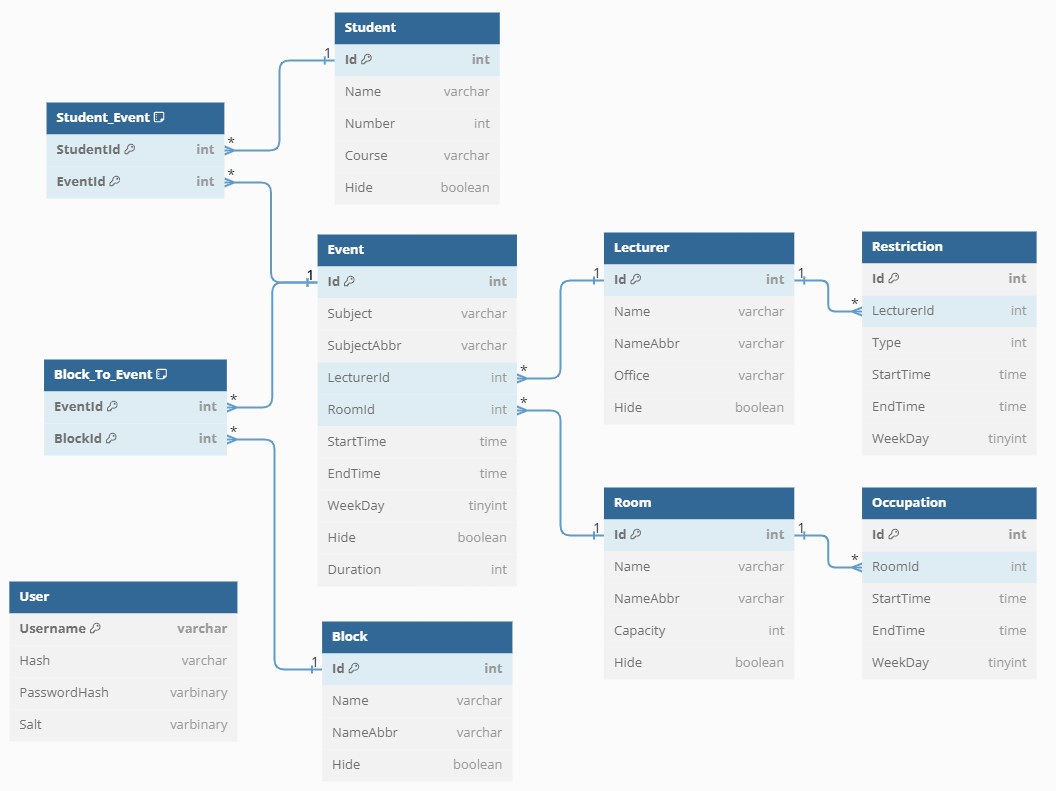
\includegraphics[width=1.1\columnwidth]{Development/uml.png}
%      \caption[UML]
%      {UML}
%      \label{fig:uml}
%\end{figure}
% Tests

% Main chapter title
%\chapter[toc version]{doc version}
\chapter{Tests}


\label{Tests}

This chapter outlines the numerous tests used to evaluate the performance of the final algorithm on instances from the \ac{itc-2007} benchmark. All the tests were executed on a computer with the following characteristics: (...)

%\section{Test Instances}

\section{Test Setup}

The tests were conducted for different values of the parameter \(C\) (Formula \ref{uct_formula}), which affects the exploration-exploitation trade-off in the \ac{mcts} algorithm. A higher \(C\) value increases the weight of the second term, allowing the algorithm explore less-visited nodes with more intensity. On the other hand, a lower \(C\) value favors nodes with a higher average reward, resulting in increased exploitation of known favorable choices. Specifically, we tested the algorithm with some values of C ranging from 0.1 to 1000.

Additionally, an alternative UCT formula was evaluated, modifying the exploitation term to use the accumulated reward instead of the average (Formula \ref{modified_uct}), giving an advantage to the nodes that were exploited first.

\begin{equation}
UCT = w_i + 2C\sqrt{\frac{2\ln{n}}{n_i}},\label{modified_uct}
\end{equation} where \(w_i\) is the total reward of all playouts through this state, \(n_i\) is the number of visits of child node \(i\), \(C\) is a constant greater than zero (typically \(\sqrt{2}\)), and \(n\) is the number of visits of the parent node.
	
	
\section{Performance Metrics}

Each test corresponds, therefore, to a different C value, and the performance measurements are recorded for 21 problem instances, denoted as comp01 to comp21. For each instance, the method iterates numerous times until a stopping condition is met, which is usually a time constraint.

For each test, the following key performance metrics were considered:

\begin{itemize}
\item \textbf{Best hard penalty:} The lowest number of hard constraint violations found during the execution of the algorithm for a given instance. A value of zero indicates a feasible solution that satisfies all hard constraints.

\item \textbf{Best soft penalty:} The lowest soft constraint penalty achieved during the search process for a given instance.

\item \textbf{Iteration of best solution:} The specific iteration at which the best solution (in terms of hard or soft penalties) was found.

\item \textbf{Total number of iterations:} The overall count of iterations performed during the algorithm's execution for each problem instance.

\item \textbf{Time to best solution:} The elapsed time required to reach the best solution for a given instance.
\end{itemize}


\section{Testing Procedure}

To thoroughly evaluate the algorithm's robustness and consistency, two different testing approaches were employed:

\begin{enumerate}

\item \textbf{Without seed (1-hour runs):} The algorithm was executed for 1 hour without a predefined random seed, allowing the algorithm to explore diverse search paths without being constrained by an initial fixed state. The goal was to assess its ability to converge towards high-quality solutions given sufficient runtime.

\item \textbf{With fixed seeds (10-minute runs):} The algorithm was run for 10 minutes using ten different seeds (1-10). Using fixed seeds ensured that the results could be reproduced, allowing for a fair comparison of different parameter settings and configurations. This approach also helped to evaluate the consistency and variability of results across different initializations. 

\end{enumrate}
\chapter{Results}

\label{Results}

This chapter presents the main outcomes of the proposed \ac{mcts}-based system for \ac{cb-ctt}, including its performance, feasibility, and evaluations of enhancements such as the diving strategy.

\section{Python vs PyPy Performance}

During the development and testing of the system, both standard Python and PyPy\footnote{A Just-In-Time (JIT) compiling alternative. Link: https://pypy.org/} were evaluated for performance. While both interpreters correctly executed the \ac{mcts} algorithm, the performance difference was substantial. PyPy called over 3 times more functions compared to Python.

Given the compute-intensive nature of \ac{mcts}, PyPy was ultimately chosen for running all the experiments and benchmarks.

\section{Feasibility}

The proposed system consistently produced feasible solutions across all tested configurations and datasets.

\section{\(C\) Parameter Behaviour}

The exploration constant \(C\) in the \ac{uct} formula (Formula \ref{uct_formula}) was varied across several orders of magnitude (from 0.1 to 1000), including the modified variant incorporating accumulated rewards (Formula \ref{modified_uct}). Surprisingly, the results showed that varying \(C\) had minimal impact on solution quality, which indicates a lower-than-expected sensitivity to node selection.

\section{Diving strategy}

\section{Competition Results Comparison}
% Conclusion

% Main chapter title
%\chapter[toc version]{doc version}
\chapter{Conclusion}

% Short version of the title for the header
%\chaptermark{version for header}

% Chapter Label
% For referencing this chapter elsewhere, use \ref{ChapterTemplate}
\label{Conclusion}

The proposed approach presents a novel application of\ac{mcts} to\ac{ucttp}, combined with\ac{hc} for local improvements. While\ac{mcts} has seen limited application in\ac{ucttp}, this dissertation demonstrates its potential.

The integration of\ac{hc} significantly improves solution quality by exploiting feasible regions more effectively.

An additional innovation is the incorporation of a diving strategy into the\ac{mcts} process. This mechanism allows the algorithm to focus more deeply on promising branches of the search tree, accelerating convergence and reducing unnecessary exploration.

However, our findings indicate that both standard and diving-based\ac{mcts} tend to plateau after a certain number of iterations, with diminishing returns even under extended run times. While diving produces more consistent improvements and tends to stay closer to the best-found solutions, the problem of long-term stagnation remains and represents a key area for future optimization.

Our experimental results, including comparisons against the benchmark dataset from the ITC-2007 competition, show that the hybrid approach consistently produces feasible solutions. Although it does not yet outperform state-of-the-art solutions, this dissertation provides an effective and adaptive scheduling process for\ac{fcup} and can be extended to other institutions and help in other studies. 

\section{Future Work}

Future work may focus on fine tuning the algorithm, improving the heuristic functions, enhancing computational performance, and integrating a visualization tool.

\subsection{Performance}

One promising direction is to postpone rooms allocation during both tree construction and simulation. In this approach, the fixed nodes in the tree represents only the \((weekday, timeslot)\) (Appendix \ref{AppendixA} Figure \ref{fig:tree}) and, in the simulation, only allocate these two attributes for each event. Room assignments are performed afterward, once the simulation reaches a complete assignment of periods. Exploring this variant could help reduce computational overhead and allow deeper or broader search within the same time constraints.

Although early testing of this approach did not yield strong results, it remains a promising idea that deserves further investigation and refinement.

\subsection{Previous Work}

A previous project\footnote{\textbf{Front-end:} \url{https://github.com/luismdsleite/schedule} \textbf{Back-end:} \url{https://github.com/luismdsleite/schedule-backend}} developed a timetabling visualization tool using Flask and reactive programming principles with the Elm language. Flask facilitated data management and communication between the front-end and the database (Appendix \ref{AppendixA} Figure \ref{fig:previous_work_uml}), ensuring that timetable updates were efficiently processed and displayed. 

This tool allows users to manually construct and modify schedules while providing a responsive interface (Appendix \ref{AppendixA} Figure \ref{fig:previous_work_interface}). However, despite its usability, the tool has some limitations that this dissertation attempted to address:

\begin{itemize}
\item \textbf{No conflict detection support:} Users had to manually check for conflicts, increasing the risk of errors.
\item \textbf{Lack of automated guidance:} It did not provide recommendations or suggestions to help users make optimal scheduling decisions.
\item \textbf{No quality assessment:} The system lacked mechanisms to evaluate the quality of a given timetable.
\end{itemize}

The development process involved several adaptations and refinements. Initially, the previous work was analyzed and made functional, serving as a baseline for the new system. 

The\ac{mcts} algorithm was being developed while also being integrated into the front-end interface intended to showcase the project. However, as the focus shifted towards adapting it to the\ac{itc-2007} track 3 benchmark for performance evaluation and fine-tuning the algorithm, the front-end development gradually lost priority. As the algorithm evolved and diverged significantly from its original form, aligning it with the prior work proved difficult. Consequently, continuing its development would be time-consuming and ultimately not worthwhile, as it was primarily intended for demonstration purposes. Instead, the system should be directly integrated into the sigarra\footnote{\url{https://sigarra.up.pt/up/pt/web\_page.inicial}} website.

%\begin{figure}
%    \centering
%      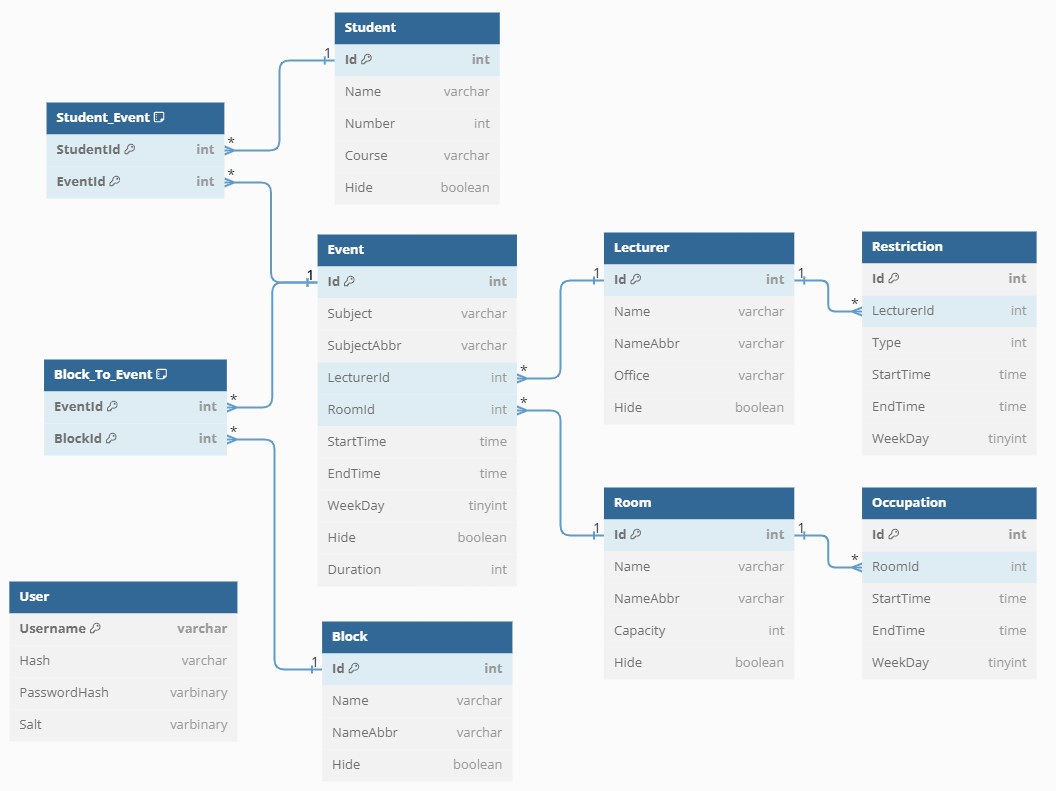
\includegraphics[width=1.1\columnwidth]{Development/uml.png}
%      \caption[UML]
%      {UML}
%      \label{fig:uml}
%\end{figure}



% Add others as needed


%-------------------------------------------------------------------------
%	BIBLIOGRAPHY
%-------------------------------------------------------------------------
\addvspacetoc{0.5cm}
\addtotoc{Bibliography}

%\fancyhead[LO]{\textsc{Bibliography}}

 % The references are stored in the file "Bibliography.bib"
\bibliography{Bibliography}

%-------------------------------------------------------------------------
%	THESIS CONTENT - APPENDICES
%-------------------------------------------------------------------------

\appendix % Cue to tell LaTeX that the following 'chapters' are Appendices

%%% -----------  ADD APPENDIX HERE ------------------ %%%

%% Appendix Template

\chapter*{Appendix} % Main appendix title

\label{Appendix1} % Change X to a consecutive letter; for referencing this appendix elsewhere, use \ref{AppendixX}

\begin{table}[!h]
    \centering
    \caption{ITC-2007 track 3 results comparison}
    \scalebox{0.7}{
    \begin{tabular}{|l|l|l|l|l|l|l|l|}
    \hline
        \multicolumn{2}{|c|}{\textbf{Instances / Competitors}} & \textbf{Müller} & \textbf{LuHao} & \textbf{Atzuna} & \textbf{Geiger} & \textbf{Clark} & \textbf{My Results} \\ \hline
        \textbf{comp01} & average & 5 & 5 & 5 & 6,7 & 27 & 26 \\
        & max & 5 & 5 & 5 & 9 & 68 & 26 \\
        & min & 5 & 5 & 5 & 5 & 10 & 26 \\ \hline
        \textbf{comp02} & average & 61,3 & 61,2 & 65,6 & 142,7 & 131,1 & 242 \\
        & max & 70 & 74 & 76 & 168 & 146 & 242 \\
        & min & 51 & 55 & 50 & 111 & 111 & 242 \\ \hline
        \textbf{comp03} & average & 94,8 & 84,5 & 89,1 & 160,3 & 138,4 & 247 \\
        & max & 103 & 101 & 95 & 188 & 167 & 247 \\
        & min & 84 & 71 & 82 & 128 & 119 & 247 \\ \hline
        \textbf{comp04} & average & 42,8 & 46,9 & 39,2 & 82 & 90,2 & 155 \\
        & max & 48 & 53 & 44 & 91 & 110 & 155 \\
        & min & 37 & 43 & 35 & 72 & 72 & 155 \\ \hline
        \textbf{comp05} & average & 343,5 & 326 & 334,5 & 525,4 & 811,5 & 763 \\
        & max & 379 & 346 & 353 & 691 & 2000 & 763 \\
        & min & 330 & 309 & 312 & 410 & 426 & 763 \\ \hline
        \textbf{comp06} & average & 56,8 & 69,4 & 74,1 & 110,8 & 149,3 & 273 \\
        & max & 65 & 80 & 84 & 129 & 181 & 273 \\
        & min & 48 & 53 & 69 & 100 & 130 & 273 \\ \hline
        \textbf{comp07} & average & 33,9 & 41,5 & 49,8 & 76,6 & 153,4 & 224 \\
        & max & 45 & 49 & 56 & 89 & 191 & 224 \\
        & min & 20 & 28 & 42 & 57 & 110 & 224 \\ \hline
        \textbf{comp08} & average & 46,5 & 52,6 & 46 & 81,7 & 96,5 & 163 \\
        & max & 55 & 58 & 50 & 90 & 116 & 163 \\
        & min & 41 & 49 & 40 & 77 & 83 & 163 \\ \hline
        \textbf{comp09} & average & 113,1 & 116,5 & 113,3 & 164,1 & 148,9 & 268 \\
        & max & 117 & 127 & 121 & 178 & 157 & 268 \\
        & min & 109 & 105 & 110 & 150 & 139 & 268 \\ \hline
        \textbf{comp10} & average & 21,3 & 34,8 & 36,9 & 81,3 & 101,3 & 201 \\
        & max & 27 & 48 & 49 & 96 & 122 & 201 \\
        & min & 16 & 21 & 27 & 71 & 85 & 201 \\ \hline
        \textbf{comp11} & average & 0 & 0 & 0 & 0,3 & 5,7 & 5 \\
        & max & 0 & 0 & 0 & 2 & 8 & 5 \\
        & min & 0 & 0 & 0 & 0 & 3 & 5 \\ \hline
        \textbf{comp12} & average & 351,6 & 360,1 & 361,6 & 485,1 & 445,3 & 845 \\
        & max & 367 & 380 & 378 & 544 & 487 & 845 \\
        & min & 333 & 343 & 351 & 442 & 408 & 845 \\ \hline
        \textbf{comp13} & average & 73,9 & 79,2 & 76,1 & 110,4 & 122,9 & 207 \\
        & max & 81 & 87 & 82 & 125 & 145 & 207 \\
        & min & 66 & 73 & 68 & 98 & 113 & 207 \\ \hline
        \textbf{comp14} & average & 61,8 & 65,9 & 62,3 & 99 & 105,9 & 214 \\
        & max & 69 & 77 & 68 & 108 & 127 & 214 \\
        & min & 59 & 57 & 59 & 90 & 84 & 214 \\ \hline
        \textbf{comp15} & average & 94,8 & 84,5 & 89,1 & 160,3 & 138 & 265 \\
        & max & 103 & 101 & 95 & 188 & 167 & 265 \\
        & min & 84 & 71 & 82 & 128 & 119 & 265 \\ \hline
        \textbf{comp16} & average & 41,2 & 49,1 & 50,2 & 92,6 & 107,3 & 228 \\
        & max & 49 & 57 & 60 & 103 & 127 & 228 \\
        & min & 34 & 39 & 40 & 81 & 84 & 228 \\ \hline
        \textbf{comp17} & average & 86,6 & 100,7 & 107,3 & 143,4 & 166,6 & 287 \\
        & max & 92 & 111 & 115 & 161 & 178 & 287 \\
        & min & 83 & 91 & 102 & 124 & 152 & 287 \\ \hline
        \textbf{comp18} & average & 91,7 & 80,7 & 73,3 & 129,4 & 126,8 & 163 \\
        & max & 102 & 93 & 80 & 145 & 142 & 163 \\
        & min & 83 & 69 & 68 & 116 & 110 & 163 \\ \hline
        \textbf{comp19} & average & 68,8 & 69,5 & 79,6 & 132,8 & 125,4 & 232 \\
        & max & 74 & 77 & 85 & 184 & 148 & 232 \\
        & min & 62 & 65 & 75 & 107 & 111 & 232 \\ \hline
        \textbf{comp20} & average & 34,3 & 60,9 & 65 & 97,5 & 179,3 & 235 \\
        & max & 44 & 72 & 71 & 109 & 201 & 235 \\
        & min & 27 & 47 & 61 & 88 & 144 & 235 \\ \hline
        \textbf{comp21} & average & 108 & 124,7 & 138,1 & 185,3 & 185,8 & 333 \\
        & max & 121 & 137 & 150 & 210 & 202 & 333 \\
        & min & 103 & 106 & 123 & 174 & 169 & 333 \\ \hline
    \end{tabular}}
    \label{results-comparison}
\end{table}
%\input{Appendices/AppendixB}
%\input{Appendices/AppendixC}

\backmatter


\end{document}
